%%%%%%%%%%%%%%%%%%%%%%%%%%%%%%%%%%%%%%%%%%%%%%%%%%%%%%%%%%%%
%%% LIVECOMS ARTICLE TEMPLATE FOR BEST PRACTICES GUIDE
%%% ADAPTED FROM ELIFE ARTICLE TEMPLATE (8/10/2017)
%%%%%%%%%%%%%%%%%%%%%%%%%%%%%%%%%%%%%%%%%%%%%%%%%%%%%%%%%%%%
%%%
%%% PLEASE COMPILE USING LUALATEX.
%%%
%%% PREAMBLE
\documentclass[9pt,tutorial]{livecoms}
% Use the 'onehalfspacing' option for 1.5 line spacing
% Use the 'doublespacing' option for 2.0 line spacing
% Use the 'lineno' option for adding line numbers.
% Use the "ASAPversion' option following article acceptance to add the DOI and relevant dates to the document footer.
% Use the 'pubversion' option for adding the citation and publication information to the document footer, when the LiveCoMS issue is finalized.
% The 'bestpractices' option for indicates that this is a best practices guide.
% Omit the bestpractices option to remove the marking as a LiveCoMS paper.
% Please note that these options may affect formatting.

\usepackage[version=4]{mhchem}
\usepackage{siunitx}
\DeclareSIUnit\Molar{M}
\usepackage[italic]{mathastext}
\graphicspath{{figures/}}
\usepackage{upgreek} 
\usepackage{subcaption}
\usepackage{todonotes}
\usepackage{natbib}
\usepackage{tabularx}
\usepackage{booktabs}
\usepackage{pifont}
\usepackage{wasysym}
\usepackage{ulem}
\definecolor{color-3}{rgb}{1,0,0}
\newcommand{\checkref}[1]{\uline{\emph{{\color{LiveCoMSDarkBlue}#1}}}}
%\newcommand{\checkref}[1]{{\color{LiveCoMSDarkBlue}#1}}

%%%%%%%%%%%%%%%%%%%%%%%%%%%%%%%%%%%%%%%%%%%%%%%%%%%%%%%%%%%%
%%% IMPORTANT USER CONFIGURATION
%%%%%%%%%%%%%%%%%%%%%%%%%%%%%%%%%%%%%%%%%%%%%%%%%%%%%%%%%%%%

\newcommand{\versionnumber}{1.0}  % you should update the minor version number in preprints and major version number of submissions.
\newcommand{\githubrepository}{\url{https://github.com/asmunder/BPIPMDS}}  %this should be the main github repository for this article

%%%%%%%%%%%%%%%%%%%%%%%%%%%%%%%%%%%%%%%%%%%%%%%%%%%%%%%%%%%%
%%% ARTICLE SETUP
%%%%%%%%%%%%%%%%%%%%%%%%%%%%%%%%%%%%%%%%%%%%%%%%%%%%%%%%%%%%
\title{A Guide to Computing Interfacial Properties from Molecular Simulations [Article v\versionnumber]}

\author[1*]{Erich A. M\"{u}ller}
\author[2*]{\AA{}smund Ervik}
\author[3*]{Andres Mej\'{i}a}
\affil[1]{Department of Chemical Engineering, Imperial College London, United Kingdom}
\affil[2]{Department of Gas Technology, SINTEF Energy Research, Trondheim, Norway}
\affil[3]{Departamento de Ingenier\'{i}a Qu\'{i}mica, Universidad de Concepci\'{o}n, Chile}

\corr{e.muller@imperial.ac.uk}{EAM}  % Correspondence emails.
\corr{asmund.ervik@sintef.no}{\AA{}E}
\corr{amejia@udec.cl}{AM}

\orcid{Erich A. M\"{u}ller}{0000-0002-1513-6686}
\orcid{\AA{}smund Ervik}{0000-0003-1073-887X}
\orcid{Andres Mej\'{i}a}{0000-0001-7238-6633}

\blurb{This LiveCoMS document is maintained online on GitHub at \githubrepository; to provide feedback, suggestions, or help improve it, please visit the GitHub repository and participate via the issue tracker.}

%%%%%%%%%%%%%%%%%%%%%%%%%%%%%%%%%%%%%%%%%%%%%%%%%%%%%%%%%%%%
%%% PUBLICATION INFORMATION
%%% Fill out these parameters when available
%%% These are used when the "pubversion" option is invoked
%%%%%%%%%%%%%%%%%%%%%%%%%%%%%%%%%%%%%%%%%%%%%%%%%%%%%%%%%%%%
\pubDOI{10.XXXX/YYYYYYY}
\pubvolume{<volume>}
\pubissue{<issue>}
\pubyear{<year>}
\articlenum{<number>}
\datereceived{Day Month Year}
\dateaccepted{Day Month Year}

%%%%%%%%%%%%%%%%%%%%%%%%%%%%%%%%%%%%%%%%%%%%%%%%%%%%%%%%%%%%
%%% ARTICLE START
%%%%%%%%%%%%%%%%%%%%%%%%%%%%%%%%%%%%%%%%%%%%%%%%%%%%%%%%%%%%

\begin{document}

\begin{frontmatter}
\maketitle

\begin{abstract}
Molecular simulation is ideally suited to explore and describe the behavior of
inhomogeneous fluid mixtures as it allows a unique perspective into the physics
at the scale relevant to interfacial properties, filling the gaps between
experimental determinations and theoretical predictions. Although
rather common Molecular Dynamics and Monte Carlo
schemes are employed, the technical implementation and the post-processing of the results
are more challenging than for homogeneous fluids due to the spatial dependence
of the interfacial properties. The aim of this work is to provide a guide
to molecular-simulation computation of the most important interfacial properties
of pure fluids and fluid mixtures, \textit{i.e}., interfacial concentration of
species, the interfacial thickness, the surface activity or adsorption of
species, superficial enthalpy and entropy, wetting between phases and the
interfacial or surface tension. Herein, a detailed description is given
of the steps required to perform classical molecular simulations including
setting up of the initial configuration, choice of cell dimensions, thermodynamic conditions
and ensemble, selection of the force field, simulation length, etc.
and a discussion of the required post-processing steps in order to
obtain interfacial properties. Additionally, general background and description
of the expected results of interfacial fluid properties are provided.   
\end{abstract}

\end{frontmatter}

\section{Introduction}


%Keep in mind, as you prepare your manuscript, that you should plan for a representative image  which will be used to highlight your article on the journal website and publications. Usually, this would be one of your figures, but it must also be uploaded separately upon article submission. We give specific guidelines for this image on the journal website in the section on article submission (see \url{https://livecomsjournal.github.io/authors/policies/index.html#article-submission}).
The term "interfacial properties" refers to the fundamental thermophysical
properties that govern the behaviour of inhomogeneous fluids. The defining
attribute of these systems is the existence of a boundary or interface,
spanning only a few nanometers, but across which there are typically large
changes in the local conformation of the fluids. The presence of this boundary
region plays a central role in natural, environmental, and industrial
processes. The most representative of these interfacial properties are the
concentration profiles of the species across the interface, the actual extent
(thickness) of the interfacial region, the surface activity or adsorption of
species at the interface, the superficial enthalpy and entropy, the wetting
between phases, and last, but not least, the interfacial or surface tension.
Some of these properties can be directly measured (\textit{e.g}., interfacial
thickness, wetting and interfacial/surface tension) \citep{evans2006}
whereas others must be inferred from direct measurements, albeit
usually with a high level of accuracy. 

Molecular theories for interfacial properties are well developed, usually based
on classical density functional theory \citep{evans1992,rowlinson1982}, including the van der Waals square gradient
theory \citep{davis1982,rowlinson1982}.
These theories have been shown to provide accurate results for both simple and
complex mixtures, but inevitably need extraneous information regarding
interfacial properties to be effectively used as correlation tools.

On the other hand, molecular simulation is particularly well posed to study
physical phenomena at the fluid interfaces. In these scenarios, while the
perturbations caused by the fluid heterogeneities typically extend for several
nanometers, rarely do the correlations in the neighbouring bulk phase fluid
span distances larger than 50 nm. These are the system sizes which we are
comfortable simulating with commonly available modern computers (and
clearly this will only improve with time). This accessibility of the size and
length scales pertinent to fluid interfaces has spawned in the recent past decades a surge in studies
on the computational aspects of the interfacial
tensions of pure fluids and mixtures, including the effects of third players
(surfactants, nanoparticles, etc.) 

The interfacial tension is typically not affected by the dynamics nor the prior
history of the system \footnote{The term "dynamic" interfacial tension
refers to the scenarios where the tension changes with the observation time.
These are not equilibrium conditions, but rather situations where the
properties of the interfacial region are continually evolving, typically due to
the slow mass transfer to/from the interfacial region of a third component,
\textit{e.g}., a surfactant. We will not be covering these aspects in this
manuscript. See for example \citet{dukhin1995}.}, \citep{rowlinson1982}, hence it is amenable to be computed on
the basis of an ensemble average of appropriate configurations. Both Molecular
Dynamics (MD) \citep{allen2017} and Monte Carlo (MC) \citep{frenkel2002} methods can be employed
with equal success to generate these configurations and this review makes
little distinction between both strategies, as the tensions are calculated
post-simulation by making suitable calculations on these configurations. MD has
been used more extensively than MC in recent years, as MD has benefitted from
advances in parallel computing and the use of graphical processing units \citep{faraday2014}.

The main advantage of classical molecular simulation (MS) for studying
interfacial fluids is the explicit representation of the molecules in an
environment which is commensurate with the dimension of the interfacial region
of fluids (${\simeq}$ 10 to 100 \AA{}). The interfacial regions are
characterized by sharp changes in densities and compositions, and these have to
be considered explicitly, hence the overall system sizes, in terms of number of
particles, can easily reach $O$(10$^{5}$), which is considerably more
than what is typical in single phase studies. Notwithstanding, the increasing
power of computers and the improvement in speed of the available MS packages
mean that evermore, this region of matter can be studied with increased
scrutiny. Starting with the seminal publications on MS of interfacial
properties from the middle of '70s \citep{liu1974}, several
authors have included in their manuscripts guidelines for obtaining meaningful
calculations. However, these guidelines are dispersed and sometimes differ from
author to author. The main goal of this manuscript is to provide a general,
self-contained and unified guide to perform a MS for calculating
interfacial properties of fluids using MD or MC. We do this by carrying out an
exemplary MS of an inhomogeneous fluid detailing the advice with regards to the
set-up, running and data analysis. In this work, we are focused on MS for
computing interfacial properties of pure fluids and fluid mixtures in
vapor-liquid and liquid-liquid equilibrium. 

\section{Prerequisites}
\subsection{Recommended Reading}
In addition to the recommendations, highlights and other issues concerning the
prediction of interfacial properties are described in this document; we
recommend the following textbooks and selected reviews and regular articles in
this field. 

\begin{itemize}
  \item Allen and Tildesley, \textit{Computer simulation of liquids}, 2$^{\mathrm{ed}}$. pages 84\textendash{}89 and Chap. 14. \citep{allen2017}

In this new edition of a classical textbook, the authors have included a chapter devoted to summarizing the most important aspects of carrying out MD and MC for inhomogeneous systems.

\item Gray, Gubbins, and Joslin, \textit{Theory of molecular fluids: Vol. 2: Applications}, Chap. 8. \citep{gray2011}

This book lucidly presents the principal elements of the statistical mechanics involved in the prediction of interfacial properties from MS, such as the Kirkwood pressure tensor and Test Area method.

\item Ghoufi et al., \textit{Computer modelling of the surface tension of the gas-liquid and liquid-liquid interface.} \citep{ghoufi2016}

  In this recent review the interfacial tension and related properties are calculated by using different methodologies using both MC and MD. A significant number of key references as well as previous reviews are listed within.

\item Holcomb et al. \textit{A critical study of the simulation of the liquid-vapour
interface of a Lennard-Jones fluid.} \citep{holcomb1993}

  This is a 
  seminal paper where the implementation and use of Kirkwood pressure
  tensor to calculate interfacial tension is described. Still relevant today,
  this work summarizes some important issues concerning to the impact of the
  initial condition on the results from Kirkwood pressure tensor.

\item Gloor et al. \textit{Test-area simulation method for the direct determination of the interfacial tension of systems with continuous or discontinuous potentials.} \citep{gloor2005}
  
  This manuscript presented an alternative methodology to compute interfacial tension from perturbation theory rather than the more commonly used Kirkwood pressure tensor.

\item Zhang et al., \textit{Computer simulation of liquid/liquid interfaces. I. Theory and application to octane/water.} \citep{zhang1995}

  This work enumerates and comments on the several types of molecular ensembles available to carry out MS of interfacial tensions.

\item Additionally, references \citep{walton1983,chapela1977,trokhymchuk1999,mecke1997,mecke1999,duque2004,errington2007,stephan2019} are a few
  selected articles where the calculation of interfacial density (or
  concentration) and interfacial tension for pure fluids and fluid mixtures are
  described with emphasis on either methodology or reference fluid results. 

\end{itemize}

\subsection{Software}
There is
a spectrum of molecular simulation packages to choose from
in order to carry out molecular simulations of inhomogeneous fluids,
ranging from commercial and academic
versions to homemade codes. Most of them have a built-in subroutine to
calculate the density or concentration along the interfacial region but rarely
is there built-in provision to calculate interfacial/surface tension. This
interfacial property should be calculated by modifying the original code or
computed in a post-processing step as will be described later. Table
\ref{tab:1} summarizes some examples of the molecular simulation packages frequently
employed in academia for describing interfacial properties of fluids. In
general terms, MD software is available in parallelized versions, capable of
running on multiple CPUs (and/or multiple GPUs) whereas MC software is normally
only available in serial versions. The corresponding websites of these
simulation packages typically include the user manual, some examples of the input
files and output files as well as some benchmarks. The reader is redirected to
Ref. \citep{wiki} for a general classification of MS software. 


The selection of a simulation package is to some extent a personal decision,
influenced by the general environment (\textit{i.e.}, available support ) and
familiarity. For most simulations described here, the programs have been
tested, validated and debugged (see however section \ref{sec:bugs}). For research
applications it is well advisable to select a program written in a language
which is familiar to the user, as most likely some level of modification will eventually
be needed. In this regard, and with no prejudice, DL\_POLY is an exemplary
choice as its codes are written in a clear, modular, style providing for
a reasonably straightforward way to implement additional subroutines. Speed of
execution is also an important consideration, and there can be significant
differences between the different compiled programs. In addition to calculation
software, MS typically uses extra programs for three purposes: to setup initial configurations
(\textit{i.e}., molecular editor), to plot resulting tabular data like such as 
time evolution of temperature and pressure, and to visualize 
spatial configurations and their temporal evolution. Some selected examples are
the Avogadro \citep{avogadro}, xmgrace \citep{xmgrace},
VMD \citep{VMD}, Ovito \citep{ovito}, and PyMOL \citep{pymol} softwares.
Avogadro is a molecular editor and visualizer which can
be used to build initial configurations or to read molecular configurations in
a myriad of styles, including the NIST webbook \citep{lemmon2013}. xmgrace is a 2D graphic software with high capability to
easily read, manipulate data, compute preliminary results and plot the output
files from MS. VMD, Ovito and PyMol are 3D visualization programs useful to
produce snapshots of spatial configurations and to visualize their temporal
evolution. VMD, Ovito and PyMol can read numerous different file formats which
making them very versatile. They also include some plugins to
carry out some simpler calculations, such as computing and plotting density profiles. VMD and Ovito
are free of charge software, whereas PyMol is a commercial software and
requires an annual fee.

\begin{table}[hb]
  \caption{Summary of selected software to perform molecular simulations
    of inhomogeneous fluids. Checks (crosses) indicate the availability
    (unavailability) of provisions to output the density profile ${\rho}(z)$,
interfacial tension $\gamma$, the ensemble average of the pressure tensor
${\langle}P_{kk}{\rangle}$ and/or the ensemble average of the
pressure tensor in each slab along the $z$ coordinate
${\langle}P_{kk}$ ($z$)${\rangle}$.}
\label{tab:1}
\begin{tabularx}{\textwidth}{
p{\dimexpr 0.23\linewidth-2\tabcolsep}
p{\dimexpr 0.22\linewidth-2\tabcolsep}
p{\dimexpr 0.08\linewidth-2\tabcolsep}
p{\dimexpr 0.13\linewidth-2\tabcolsep}
p{\dimexpr 0.08\linewidth-2\tabcolsep}
p{\dimexpr 0.10\linewidth-2\tabcolsep}
p{\dimexpr 0.14\linewidth-2\tabcolsep}}
\centering\arraybackslash{}Software & \centering\arraybackslash{}Language & \centering\arraybackslash{}MS & \centering\arraybackslash{}${\rho}$ (z) & \centering\arraybackslash{}${\gamma}$ & \centering\arraybackslash{}${\langle}$P$_{\mathrm{ii}}{\rangle}$ & \centering\arraybackslash{}${\langle}$P$_{\mathrm{ii}}$(z)${\rangle}$ \\
\midrule
\href{https://www.scd.stfc.ac.uk/Pages/DL_POLY.aspx}{DL\_POLY}  & Fortran & MD & \centering\arraybackslash{}\ding{52} & \centering\arraybackslash{}\ding{56} & \centering\arraybackslash{}\ding{52} & \centering\arraybackslash{}\ding{56} \\
\href{http://www.gromacs.org}{GROMACS}   & C++ & MD & \centering\arraybackslash{}\ding{52} & \centering\arraybackslash{}\ding{52} & \centering\arraybackslash{}\ding{52} & \centering\arraybackslash{}\ding{56} \\
\href{http://glotzerlab.engin.umich.edu/hoomd-blue/}{HOOMD}     & C++ & MD & \centering\arraybackslash{}\ding{56} & \centering\arraybackslash{}\ding{56} & \centering\arraybackslash{}\ding{52} & \centering\arraybackslash{}\ding{56} \\
\href{https://lammps.sandia.gov}{LAMMPS}    & C & MD & \centering\arraybackslash{}\ding{52} & \centering\arraybackslash{}\ding{56} & \centering\arraybackslash{}\ding{52} & \centering\arraybackslash{}\ding{52} \\
\href{http://www.ks.uiuc.edu/Research/namd/}{NAMD}      & C++ & MD & \centering\arraybackslash{}\ding{52} & \centering\arraybackslash{}\ding{56} & \centering\arraybackslash{}\ding{52} & \centering\arraybackslash{}\ding{56} \\
\href{http://pagesperso.lcp.u-psud.fr/rousseau/gibbs.html}{Gibbs}\footnotemark     & Fortran & MC & \centering\arraybackslash{}\ding{52} & \centering\arraybackslash{}\ding{52} & \centering\arraybackslash{}\ding{52} & \centering\arraybackslash{}\ding{52} \\
\end{tabularx}
\end{table}
\footnotetext{The Gibbs program is commercially available as part of the Materials Design software suite \url{https://www.materialsdesign.com}}

This guide discusses the background and details of molecular simulation for computing interfacial properties over the next six sections. A checklist for performing simulations is given in Appendix \ref{checklist}.

%Here you would identify prerequisites/background knowledge that are assumed by your work and your checklist which you view as critical, ideally giving links to good sources on these topics.
%Checklists are normally focused on errors made by users with training and experience in molecular simulations, so you can assume a basic familiarity with the fundamentals of molecular simulations.
\section{General description and main equations to compute interfacial properties of fluids.}

The properties in the interfacial region are characterized by their spatial
dependence. In molecular simulations, the interfacial region is generally
described as a function of a unidimensional coordinate. For the case of planar
interfaces, the selected coordinate is $z$ which is perpendicular to the
interfacial area, here $xy$. For the case of spherical interfaces, such
as drops or bubbles, the interfacial region is generally described as
a function of a radius.

In this section, we enumerate the most common interfacial properties and the
expressions for the planar interfaces case. For a complete description of
these expressions, the reader is redirected to Refs. \citep{allen2017,gray2011}.

\subsection{Density Profiles}

Fig. \ref{fig:1} illustrates a typical density profile, ${\rho}$ ($z$), in the
$z$ direction (perpendicular to the interface plane) for a pure fluid
in a state of vapor-liquid equilibrium. A characteristic feature is the
constant density in the bulk regions of the liquid (L) and vapor (V)
(\textit{i.e}., ${\rho}$ = ${\rho}^{\mathrm{L}}$ or ${\rho}^{\mathrm{V}}$),
and  sharp, but continuous, changes along the interfacial regions. 

\begin{figure}
	\centering
  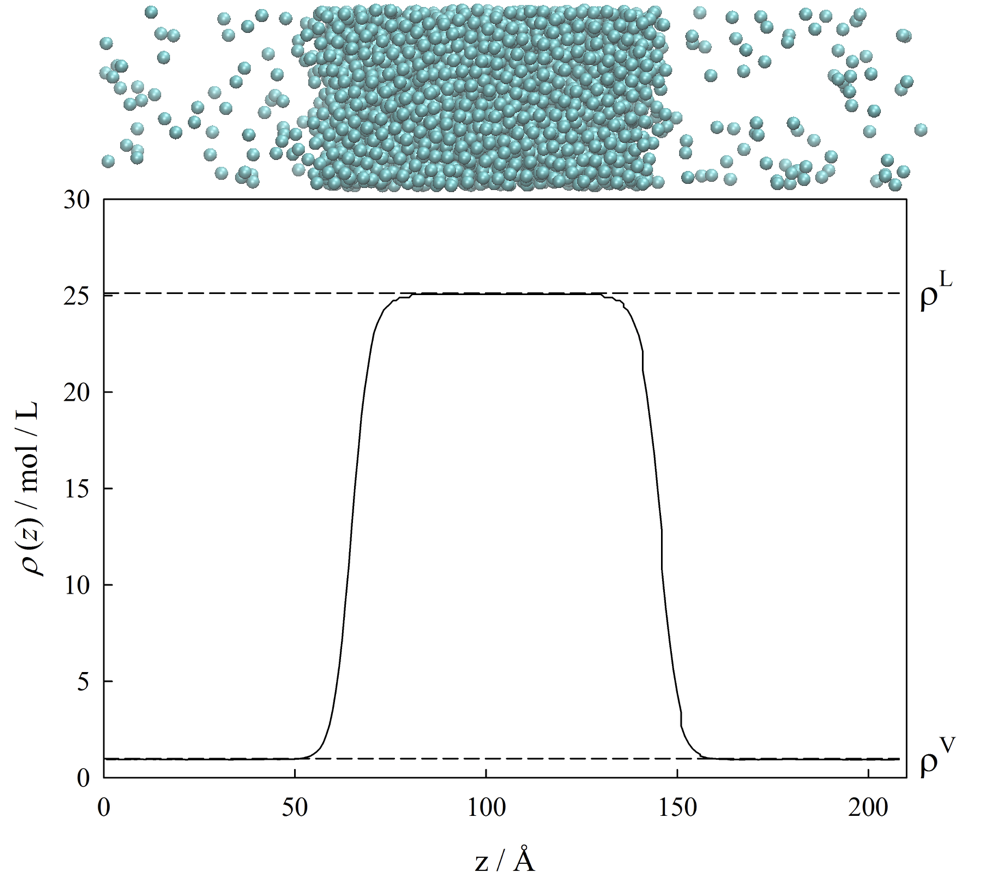
\includegraphics[width=0.4\textwidth]{gfx/image1.png}
  \caption{Density profile, ${\rho}$ (black line) against the position coordinate perpendicular to the interface ($z$) for a pure liquid CO$_{2}$ in equilibrium with its vapor at 240 K. Overlaid is a snapshot of the detail of a simulation of a liquid-vapor interface.}
  \label{fig:1}
\end{figure}

For the case of mixtures, the interfacial concentration of each component can
exhibit different patterns than those shown in Fig. \ref{fig:1}, where a simple
monotonous drift is seen in the concentration profile from a higher to a lower
density. Two other possible cases are schematically shown in Figs.
\ref{fig:2} (a) and (b). Fig. \ref{fig:2} (c) illustrates a typical example of a binary mixture
(\textit{e.g}., CO$_{2}$ + C$_{10}$H$_{22}$ at 344.15 K) where the fluid with
lower interfacial tension shows adsorption (\textit{e.g}., CO$_{2}$)

In Fig. \ref{fig:2} (a) and (b), the concentration profile displays a stationary point,
which is a maximum (point A) or a minimum (point D) of the concentration with
respect to position. Both points reflect what is referred to as \textit{surface
activity}. In general terms, surface activity refers to the accumulation (may
it be positive or negative) of a species $i$ at the interface region and
is characterized by the condition, d${\rho}_{\mathrm{i}}$/dz = 0. The
positive surface activity reflects absolute adsorption of species along the
interface region and is reflected in a negative second derivative,
d$^{2}{\rho}_{\mathrm{i}}$/dz$^{2}$ {\textless} 0. Conversely, the negative
surface activity denotes depletion of a species along the interface region, and
its condition is given by d$^{2}{\rho}_{\mathrm{i}}$ /dz$^{2}$
{\textgreater} 0. As can be appreciated, a finite surface activity implies that
the species reach higher (adsorption) or lower (desorption) concentrations than
those seen in the bulk phases. This behavior will be described latter by using
the traditional Gibbs adsorption. Additionally, Fig. \ref{fig:2} (c) shows the
concentration profiles for the case of the CO$_{2}$ + C$_{10}$H$_{22}$ mixture.
In this case, the CO$_{2}$ exhibits adsorption, where the interfacial
concentration of CO$_{2}$ is higher in the interfacial zone than bulk
concentration. This behavior is common in mixtures for the component that 
exhibits the lower interfacial tension.

\begin{figure}
	\centering
	\begin{subfigure}{0.2\textwidth} % width of left subfigure
    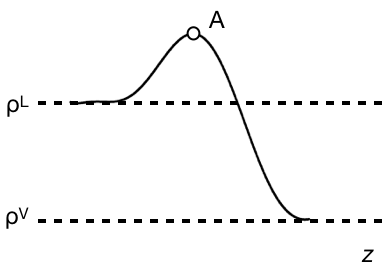
\includegraphics[width=1\textwidth]{gfx/image2.png}
		\caption{positive surface activity (adsorption)} % subcaption
	\end{subfigure}
	\hspace{1em} % here you can insert horizontal or vertical space
	\begin{subfigure}{0.2\textwidth} % width of right subfigure
    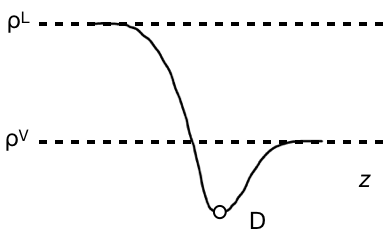
\includegraphics[width=1\textwidth]{gfx/image3.png}
		\caption{negative surface activity (desorption)} % subcaption
	\end{subfigure}
	\begin{subfigure}{0.4\textwidth} % width of right subfigure
    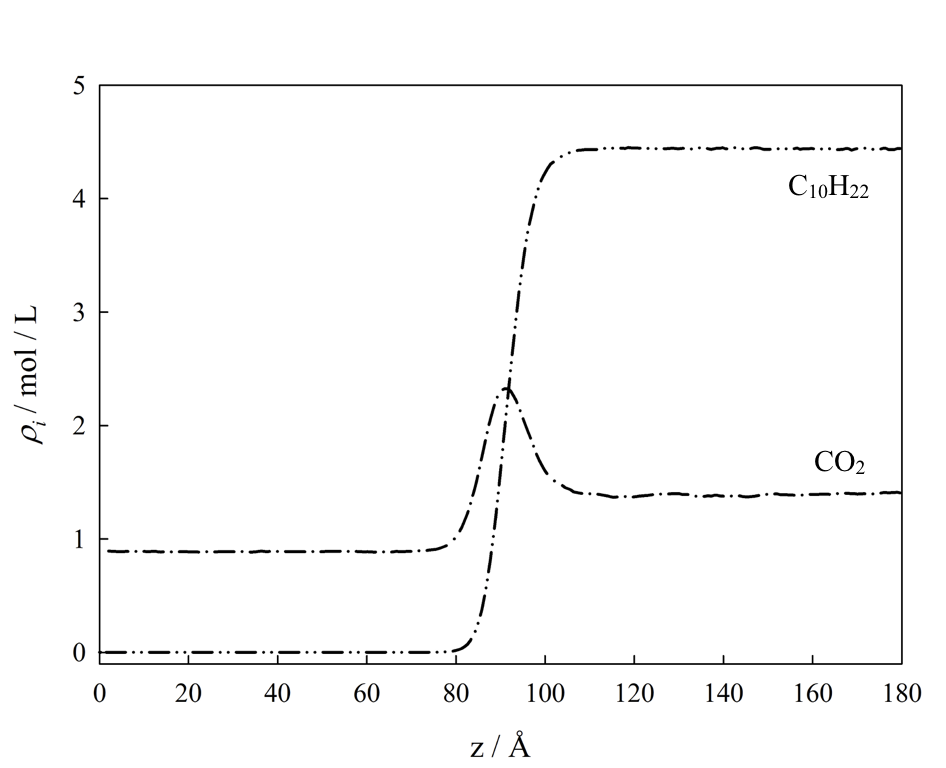
\includegraphics[width=1\textwidth]{gfx/image4.png}
		\caption{CO$_{2}$ + C$_{10}$H$_{22}$ mixture} % subcaption
	\end{subfigure}
  \caption{Concentration profiles in mixtures. (a) Schematic representation of positive surface activity (adsorption); (b) Schematic representation negative surface activity (desorption); (c) Density profile for the CO$_{2}$ + C$_{10}$H$_{22}$ mixture at 344.15 K and 2.39 MPa (cf. Example 2).} % caption for whole figure
  \label{fig:2}
\end{figure}

\subsection{Interfacial Tensions}
The interfacial (or surface) tension, $\gamma$, is arguably the best known and
most widely studied of the interfacial properties. Strictly speaking, the term
interfacial tension applies in any situation where two regions in space with
different composition and/or state are separated by a clearly defined interface
(\textit{e.g.} solid/fluid, solid/solid, fluid/fluid). Many authors let
interfacial tension refer specifically to liquid-liquid
interfaces, and let surface tension refer to gas-liquid interfaces that may be 
a liquid in contact with its own vapor phase, or with a general gas such as air.
In the context of this manuscript, the methods and discussion are more general,
and so we do not make this distinction but use the terms interchangeably.

In MS, the interfacial (or surface) tension of pure fluids and
fluid mixtures can be typically calculated from two different approaches,
namely a) the mechanical or pressure approach and b) the thermodynamic or
perturbation approach.

For an inhomogeneous fluid, the pressure is a second-order tensor \textbf{P},
where each component $P_{ij}$ gives the force per unit area in the
$j$-direction on a surface pointing in the $i$-direction. The
axial symmetry about the $z$-axis (normal to the interface) and
translational symmetry in the $xy$-plane imply that all the off-diagonal
components are zero, thus there are only two independent, non-zero components:
$P_{xx} = P_{yy} = P_T$, the tangential pressure (which changes along the
interfacial region in the $z$ direction); and the normal, or bulk
pressure $P_{N} = P_{zz} = P$ which remains constant
throughout the system, guaranteeing mechanical equilibrium. In the
pressure approach, the interfacial (or surface) tension, $\gamma$, is given by the
Hulshof integral \citep{hulshof1901}, which
is based on evaluating the inhomogeneity of the pressure tensor:

\begin{equation}
\gamma=\int_{-\infty}^{+\infty}\left[P_{N}-P_{T}\right]dz
\label{eq:hulshof}
\end{equation}

An alternative, but equally rigorous approach, recognizes that the interfacial
(or surface) tension may be expressed statistically as the difference in free energy for
systems in closely related macrostates with different interfacial areas. In
this so-called thermodynamic approach, $\gamma$ is calculated from the
following expression \citep{gray2011,gloor2005,errington2007}:

\begin{equation}
\gamma=\left(\frac{\partial F}{\partial A}\right)_{N_{i},T,V}
\label{eq:2}
\end{equation}

Where $F$ is the Helmholtz free energy of the system\footnote{
Most commonly in the engineering literature the Helmholtz free energy is symbolized by the
letter "$A$". However, in the context of this manuscript this would lead
to a confusion between this quantity and the surface area, which we label herein as
"$A$".}.  The derivative is calculated by performing an (almost)
infinitesimal perturbation in the interfacial area $A$ at canonical conditions
(keeping the compositions, volume $V$ and temperature $T$ of the
system constant). The details of the implementation of these methods is the
subject of Sec.~\ref{sec:simdetails}.

Fig. \ref{fig:3} illustrates some examples of the experimentally observed behaviour of
$\gamma$ in pure fluids and fluid mixtures. For the case of pure fluids and
zeotropic fluid mixtures in vapor-liquid equilibrium (the most common
scenarios), {${\gamma}$} decreases as temperature or pressure increases.
A similar monotonous decay can be observed with changing compositions. For the
case of azeotropic [(${\partial}$P/${\partial}$x$_{\mathrm{i}}$) = 0 or
(${\partial}$T/${\partial}$x$_{\mathrm{i}}$) = 0] or aneotropic
[(${\partial}${${\gamma}$} /${\partial}$x$_{\mathrm{i}}$) = 0] fluid mixtures,
{${\gamma}$} exhibits a stationary point [(${\partial}${${\gamma}$}
/${\partial}$x$_{\mathrm{i}}$) = 0; (${\partial}${${\gamma}$}/${\partial}$P)
= 0; (${\partial}${${\gamma}$}/${\partial}$T) = 0]. These stationary points
reflect a change of the surface activity of species $i$. These are
infrequently encountered systems and conditions, normally associated with
certain pathological types of liquid-liquid equilibria, where {${\gamma}$} shows a parabolic
behaviour with temperature or pressure.
\begin{figure}
  \centering
  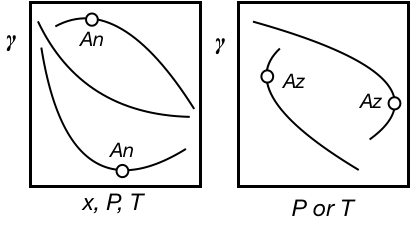
\includegraphics[width=0.4\textwidth]{gfx/image7.png}
  \caption{Schematic examples of the possible behaviour of the interfacial (or surface) tension ({${\gamma}$}) with temperature ($T$), pressure ($P$) or mole fraction ($x$) in either vapor-liquid, or liquid-liquid equilibria. $An$ refers to aneotropic points, $Az$ refers to azeotropic points.}
  \label{fig:3}
\end{figure}

A third class of methods is based on the
concepts of finite-size scaling within the grand canonical ensemble 
\citep{binder1982,errington2003}. Essentially, umbrella
sampling is used to fully sample the relevant range of values for the number of
particles $N$ present in the grand canonical system, thus providing a free-energy
density profile (which is directly related to the density profile) from where
the interfacial density may be derived. The method is particularly suitable in the vicinity of
the critical region where other methods are cumbersome to apply, but its
implementation \cite{allen2017,schrader2009} will not be discussed
herein.

\subsection{Derivative interfacial properties}

The density (or concentration) profiles along the interfacial region,
${\rho}_{i}$ ($z$), and the interfacial (or surface) tension,
{${\gamma}$}, are by far the most reported of the thermophysical properties of
fluid interfaces. Aside from their own inherent value, these properties provide
a route to calculate others descriptors of the interface such as the
interfacial thickness, {${\delta}$}, the relative Gibbs adsorption isotherm,
${\Gamma}_{ij}$, the change of surface entropy
, ${\Updelta}s^{{\gamma}}$, and surface enthalpy
, ${\Updelta}h^{{\gamma}}$, and the critical temperature of pure
fluids, $T_{c}$, as we describe below. 

\subsubsection{The density profile and interfacial thickness}

The interfacial thickness $\delta$ is defined as the width of the region where observable properties such as
density change with the spatial coordinate. The range of the interfacial
thickness typically oscillates between 10 to 200 \AA{} at subcritical conditions and has
an exponential increase with temperature. As the system tends to the critical
state, the width diverges, {${\delta}$} ${\rightarrow}{\infty}$. Clearly, as
the continuous nature of the density (composition) variation precludes any
unique definition of where the bulk region ends and where the interface itself
dominates, some arbitrary criterion must be invoked. A popular choice is the so-called
10/90 criteria. Within this definition, {${\delta}$} represents the
$z$ range where the density profile changes from
${\rho}^{\mathrm{{\upalpha}}} + 0.1({\rho}^{\mathrm{{\upbeta}}}
- {\rho}^{\mathrm{{\upalpha}}}$) to
${\rho}^{\mathrm{{\upalpha}}} + 0.9 ({\rho}^{\mathrm{{\upbeta}}}
- {\rho}^{\mathrm{{\upalpha}}}$), where
${\rho}^{\mathrm{{\upalpha}}}$ and ${\rho}^{\mathrm{{\upbeta}}}$ are the bulk
densities in the {${\alpha}$} and {${\beta}$} phases, respectively.

For the case of pure fluid, {${\delta}$} can be calculated by fitting the following expression to the density profile\citep{evans1992,rowlinson1982}:
\begin{equation}
\rho\left(z\right)=\frac{1}{2}\left(\rho^{\alpha}+\rho^{\beta}\right)-\frac{1}{2}\left(\rho^{\alpha}-\rho^{\beta}\right)tanh\left[\frac{\theta\left(z-z_{0}\right)}{\delta}\right]
  \label{eq:3}
\end{equation}
where $\rho^\alpha$ and $\rho^\beta$ are the densities of the bulk phases with 
$\rho^\alpha > \rho^\beta$; $z_{0}$ is a reference coordinate, which is usually taken as the
mean interface or the position of the Gibbs dividing surface (see next
section) and {${\uptheta}$} = 2 tanh$^{-1}$ 0.8 = 2.19722; this latter value
chosen so that {${\delta}$} can be defined as the 10/90 interfacial thickness.

The use of the $\tanh$ (or equivalent fitting function such as $\mathrm{erf}$) suggests
that one could express the adsorption (or depletion) of a species as the
difference between the pointwise composition (or density) and that of the bulk
regions. The relative Gibbs adsorption isotherm of a species $i$
relative to a species $j$ (${\Gamma}_{ij}$ ) can be thus defined in
terms of ${\rho}_{i}$ ($z$) by the following integral
equation \citep{rowlinson1982}:
\begin{equation}
\varGamma_{ij}=\int_{-\infty}^{z_{0}^{j}}\left[\rho_{i}\left(z\right)-\rho{}_{i}^{\alpha}\right]dz+\int_{z_{0}^{j}}^{+\infty}\left[\rho_{i}\left(z\right)-\rho{}_{i}^{\beta}\right]dz
 \label{eq:4}
\end{equation}

In Eq. \ref{eq:4}, $z_{0}^{\mathrm{j}}$ is the transition point between the two bulk
phases and corresponds to the position of the Gibbs dividing surface relative
to a species $j$. $z_{0}^{\mathrm{j}}$ is calculated from Eq. \ref{eq:4}
considering that species $j$ does not have adsorption along the
interfacial region, \textit{i.e}., $z_{0}^{\mathrm{j}}$ is solved for the
case that ${\Gamma}_{jj}$ = 0. Mathematically, $z_{0}^{\mathrm{j}}$ is
given by the expression:
\begin{equation}
z_{o}^{j}=\frac{\int_{-\infty}^{+\infty}\rho_{j}\left(z\right)dz}{\rho_{j}^{\alpha}-\rho_{j}^{\beta}}
\end{equation}

Fig. \ref{fig:4} (a) illustrates this construction, which essentially maps the areas
between the smooth density profile and a hypothetical infinitely steep (and
thin) interface in such a way that the dividing surface corresponds to the
average interface. If there is more than one component in the system, the
Gibbs dividing surface for component $j$ does not need to correspond
a point of average null adsorption for other components. As seen in Fig. \ref{fig:4} (b),
another component $i$ in the mixture may display adsorption at the
interface relative to a species $j.$

\begin{figure}
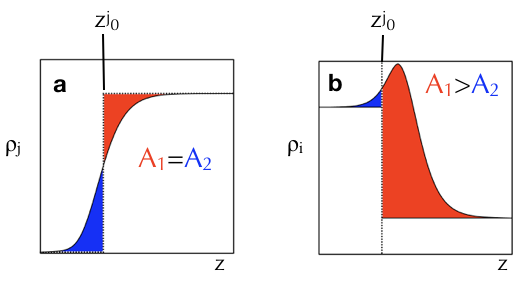
\includegraphics[width=0.5\textwidth]{gfx/image11.png}
\caption{(a) Schematic position of the Gibbs dividing surface $z^{j}_{0 }$calculated by selecting the point of no adsorption, ${\Gamma}_{jj}$ = 0, where the areas above and below the density profile cancel out. (b) For other components $i$  in the mixture, this Gibbs dividing surface suggests the adsorption of a species $i,{\Gamma}_{ij}$ {\textgreater} 0.}
\label{fig:4}
\end{figure}

\subsubsection{The surface entropy and surface enthalpy}

The entropy (${\Updelta}s^{{\gamma}}$) and enthalpy
(${\Updelta}h^{{\gamma}}$) change of surface formation can be
calculated from the following derivative expressions which are related to
{${\gamma}$} \citep{rowlinson1982}: 
\begin{equation}
  \Delta s^{\gamma} =-\left(\frac{\partial\gamma}{\partial T}\right)_{P,x} \\
  \label{eq:6}
\end{equation}
\begin{equation}
  \Delta h^{\gamma} =\gamma+T\Delta s^{\gamma}
  \label{eq:7}
\end{equation}
These quantities cannot be directly measured, but are inferred from surface tension isotherms.

\subsubsection{Critical temperature of a pure fluid}

Although not strictly an interfacial property, the value of the critical
temperature of a pure fluid$, T_{c, }$can be conveniently estimated by
extrapolating the thermal evolution of the interfacial tension (${\gamma}$
\textendash{} $T$) and employing scaling laws. For the
case of ${\gamma}$, the following expression holds \citep{rowlinson1982}
\begin{equation}
\gamma=\gamma_{0}\left(1-\frac{T}{T_{c}}\right)^{1.26}
\label{eq:8}
\end{equation}
where ${\gamma}_{0}$ and $T_{c}$ are treated as unknown constants,
and their values are found by fitting the interfacial tension data with
temperature.

\section{Initial setup of the simulation}
\label{sec:setup}
\subsection{Shape of the simulation cell}

The system sizes for the MS of interfacial systems are necessarily larger than
their pure phase counterparts (or the vapor-liquid equilibrium if one considers
Gibbs Ensemble MC simulations), as one must simultaneously track two bulk phases and two
interfacial regions at the same time. In order to guarantee the simultaneous
formation of two bulk phases (\textit{e.g}., vapor and liquid or liquid and
liquid) and the interfacial region, it is customary to use a rectangular
parallelepiped simulation cell, where one Cartesian direction is larger than
the other two. By employing this geometry, one forces the appearance of slabs
of liquid and vapor ( or liquid 2 ) sandwiched side by side. The system will
spontaneously form the interfaces spanning the minimal area, parallel to the
$xy$ plane. The volume of the simulation box, $V$, is given by
$L_{x}L_{y}L_{z}$, where $L_{x}$
= $L_{y}$ and $L_{z}$ {\textgreater}{\textgreater}
$L_{x}$. Due to the periodic boundary conditions, each bulk phase is
bounded by two independent interfaces. The periodic boundary conditions in $xy$ directions
allow for conditions representative of essentially infinite interfaces. The use of
small systems and/or cubic geometries risks the formation of bubbles/drops or
similar bridges between clusters of molecules and their periodic
images\footnote{In some cases, this may actually be the desired outcome.
For example in the study of the interfacial tension of drops and bubbles,
relatively large cubic boxes are employed, where a drop/bubble forms 
far away from its periodic images. See for example \citep{lau2015}}.

Standard practice is to make the box large (and elongated), as a rule of thumb one can consider
$L_{x}$ = $L_{y}$ {\textgreater} 10 times the molecular
diameter (or bead diameter) and $L_{z}$ 3 to 8 times
$L_{x}$. These values are chosen with the purpose to accommodate
enough molecules to ensure sensible-sized bulk phases and the corresponding two
interfacial regions. 

\subsection{Initial setup of the simulation cell}

To perform the inhomogeneous simulation, one must place in the simulation cell
both phases in intimate contact. A na\"{i}ve and impractical way is to
pre-equilibrate the coexisting phases at the approximate conditions of
temperature, density and composition and build a composite box by joining both
pre-equilibrated boxes. Although possible, this strategy is not trivial to
implement, in particular when dealing with complex molecules, as the periodic
boundary conditions must be unravelled and the interface region is prone to
have overlaps between the cojoined boxes. There are two practical ways around
this problem, the volume expansion or the temperature quench methods. 

\begin{figure}[h]
\centering
	\begin{subfigure}{0.11\textwidth} % width of left subfigure
    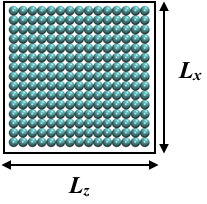
\includegraphics[width=\textwidth]{gfx/image16.png}
		\caption{Initial $\qquad$ configuration} % subcaption
	\end{subfigure}
	\begin{subfigure}{0.31\textwidth} % width of left subfigure
    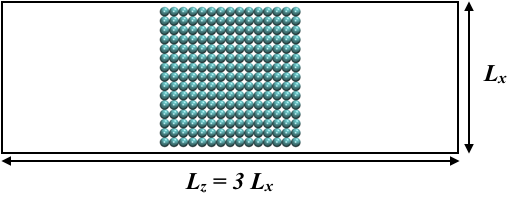
\includegraphics[width=\textwidth]{gfx/image17.png}
    \caption{Volume quench}
	\end{subfigure}
	\begin{subfigure}{0.4\textwidth} % width of left subfigure
    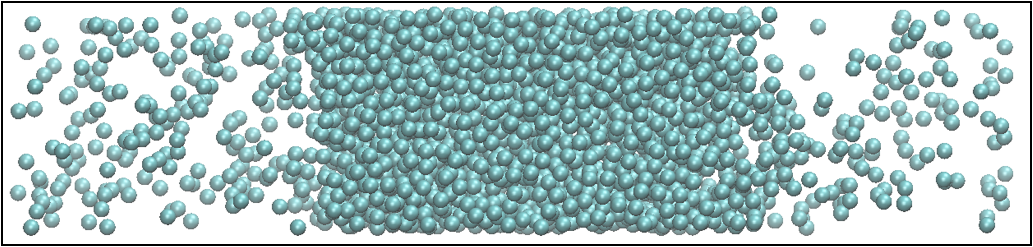
\includegraphics[width=\textwidth]{gfx/image18.png}
    \caption{Final configuration}
	\end{subfigure}
  \caption{Initial configurations for the volume expansion method. (a) An initial
cubic simulation box is set up with the density close to that of the expected
liquid phase. Molecules may be in a lattice position, randomly placed or can be
the output of an equilibrated pure fluid simulation. (b) The simulation box is
expanded in the z direction, leaving empty spaces on both sides. (c) Upon
further equilibration, some of the liquid phase molecules will evaporate,
filling the void space until the vapor pressure is attained.}
\label{fig:5}
\end{figure}

In the volume expansion ( or volume quench \citep{holcomb1993} ) case,
an initial ensemble of molecules is placed,  usually in a cubic periodic box,
in a lattice configuration or randomly distributed within the simulation cell.
The dimension of the simulation box can be set by specifying the number of
molecules desired (see below) and the expected liquid density. Once the system
equilibrates to the required temperature, two empty boxes are included at both
z-sides, making the final dimension box equal to $L_{x}
\times L_{x} \times$(3 to 8)$L_{x}$. This procedure is illustrated in Fig. \ref{fig:5}.
A further equilibration will
allow some of the liquid molecules to evaporate and fill the void regions until
the equilibrium vapor pressure is attained. This technique is particularly
suited for the case of vapor-liquid equilibria of single site molecules
(spheres) at low temperatures. 


\begin{mdframed}[linewidth=0pt,backgroundcolor=LiveCoMSLightBlue!8,fontcolor=LiveCoMSDarkBlue!80!black]
\textbf{EXAMPLE 1:} \textbf{\textit{Selection of simulation box size and number of particles for a volume expansion.}}

As an example, let us consider the MS for pure CO$_{2}$ at 240 K in the liquid
state. For this case, CO$_{2}$ will be represented by a single sphere (Mie
potential) of diameter of {${\upsigma}$} = 3.741 \AA{} \citep{avendano2011}. We take a total of 3200 spheres
and using the expected liquid density, ${\rho}$ = 24.742 mol/L \citep{lemmon2013}:
\begin{eqnarray}
  V & = & \frac{\left(3200\,\textrm{particles}\right)\left(10^{10}\right)^{3}\left(\frac{\textrm{Å}}{m}\right)^{3}}{24.742\left(\frac{mol}{L}\right)\left(N_{av}\right)\left(\frac{\textrm{molecules}}{mol}\right)\left(1000\right)\left(\frac{L}{m^{3}}\right)}\nonumber\\
  & = & 214770\textrm{Å}^{3}
\end{eqnarray}
where N$_{\mathrm{av}}$ = 6.022 . 10$^{23}$ is Avogadro's constant. Using the
value of the expected volume and a cubic cell, its vertex will be
$L_x = \sqrt[3]{V} = $ 59.886 \AA{}, which is larger than 10 $\sigma$  (37.41
\AA{}). 
\end{mdframed}

There are many instances where the volume expansion technique is not practical,
notably liquid-liquid equilibria, systems with high vapor pressures (where
a significant portion of the liquid will need to evaporate), mixtures with
large number of components, etc.  An alternative is to design the simulation
cell from the onset as a rectangular parallelepiped with $L_{x} \times L_{x} \times$(3 to 8)$L_{x}$. In order to define the
$L_{x}$ dimension, an average \textit{global} density of the fluid is
used. As an example, for the case of liquid-vapor system, the initial density
average is ${\rho}$ = (${\rho}^{\mathrm{V}}$
+ ${\rho}^{\mathrm{L}}$)/2\textit{.} Using this value of density and the
number of molecules, $M$, it is possible to calculate the total volume,
$V$ ($V$ = $M/\rho$) and $L_{x}$
= ($V$/(3 to 8))$^{\mathrm{1/3}}$. This initial configuration is
simulated at high temperature (above the critical state) to homogenize the
system. After a few steps (\textit{e.g}., 50 000 steps), the temperature of the
simulation is abruptly scaled to the final temperature (hence the name of
temperature quench \citep{martinez2005}).  If the initial
density is chosen appropriately, the system is left in a state of mechanical
instability and separates into coexisting equilibrium phases, equilibrating by
diffusion, as shown in Fig. \ref{fig:6b}.

\begin{figure}
  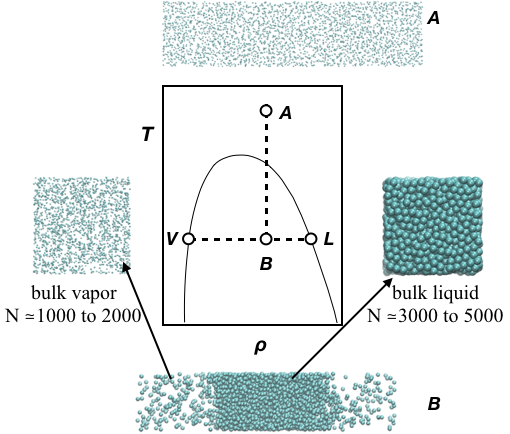
\includegraphics[width=0.5\textwidth]{gfx/image19.png}
  \caption{Preparation of the initial box. In the temperature quench strategy, one starts with a system with overall initial density and temperature such that the system is in a one phase mixed state (point A). Upon a rapid decrease in temperature, the system becomes trapped in a metastable state (B) where it spontaneously separates into two distinct phases ( V \& L ). }
  \label{fig:6b}
\end{figure}

%\begin{figure}
%	\centering
%	\begin{subfigure}{0.3\textwidth} % width of left subfigure
%    
\includegraphics[width=1\textwidth]{gfx/image20.png}
%	\end{subfigure}
%	\begin{subfigure}{0.3\textwidth} % width of left subfigure
%    
\includegraphics[width=1\textwidth]{gfx/image21.png}
%	\end{subfigure}
%  \caption{
%    Top: three typical pitfalls which are apparent from a density profile:
%    (a) insufficient statistics in the vapor region. The box should be longer to have room for the vapor phase. 
%    (b) the liquid slab does not show a plateau corresponding to a bulk liquid. Instead it shows two interfaces merging. This is resolved by increasing the average density of the system.
%    (c) the appearance of a drop outside the liquid slab. The simulation must be repeated, or run for a longer time.\\
%    Bottom: a density profile which shows a correct outcome.
%  }
%\label{fig:7b}
%\end{figure}

In either case mentioned above, the final outcome is an elongated simulation
box with slabs containing the two coexisting phases. A point to consider is the
use of an appropriate number of particles to describe not only the liquid and
vapor (or second liquid) bulk phases but also the interfacial region. The
resulting density profiles should show significant flat density regions for
each bulk phase and sufficient molecules in the sparse (vapor) phases to
provide for adequate statistics. Sec. \ref{sec:init-dens} discusses some typical
pitfalls.

For the case of pure fluids in vapor \textendash{} liquid equilibria, it is not
necessary to specify the values of $N^{L}$ and $N^{V}$, it is
only necessary to define $N^{T}= N^{L}+ N^{V}$,
as the system naturally evolves to the liquid-vapor distribution. For the case
of fluid mixtures in vapor \textendash{} liquid equilibria, it is necessary to
take into account the total number of particles for each component in all
phases (\textit{i.e}., $N_{i}^{T}$ = $N_{i}^{L}$
$+ N_{i}^{V}$). In order to calculate $N_{i}^{T}$, it is
advised to consider not only the total number of particles in each phase
($N^{L}$ and $N^{V}$) but also their composition. The
compositions in $N^{L}$ and $N^{V}$ are given by the
corresponding mole fractions in the liquid ($x_{i}$) and vapor
($y_{i}$) state. The same idea can be applied for the case of mixtures
in liquid-liquid equilibria.

\begin{mdframed}[linewidth=0pt,backgroundcolor=LiveCoMSLightBlue!8,fontcolor=LiveCoMSDarkBlue!80!black]
  \textbf{EXAMPLE 2: \textit{Selection of simulation box size and number of particles for a mixture}}

Let us to consider a CO$_{2}$ (1) + n-C$_{10}$H$_{22}$ (2) mixture at 344.15
K and 3.47 MPa. The available information \citep{shaver2001} suggests that at these
conditions, the expected mole fraction in the liquid and vapor phases are
$x_{1}$ = 0.262 and $y_{1}$ = 0.994, respectively, and the
mass densities of the phases are ${\rho}^{V}$ = 62.9 kg/m$^{3}$ and
${\rho}^{L}$ = 698.7 kg / m$^{3}$. Considering the mole fractions and the
molecular weight for the pure fluids (M$_{\mathrm{w}}$CO$_{2}$ = 44.01
kg/kgmol, M$_{\mathrm{w}}$C$_{10}$H$_{22}$ = 142.282 kg/kgmol), the average molecular
weight of the mixture in the liquid and vapor phase are M$_{\mathrm{w}}$liquid
= 116.535 kg/kgmol and M$_{\mathrm{w}}$vapor = 44.6 kg/kgmol, respectively.
Therefore, the molar densities of the mixture are  ${\rho}^{V}$ = 1.410 mol/L
and ${\rho}^{L}$ = 5.996 mol/L, hence (${\rho}^{V}$ + ${\rho}^{L}$)/2
= 3.703 mol/L.

Fluids can be described with coarse grained potentials, where CO$_{2}$ is
modelled as a single sphere ${\sigma}_{1}$ = 3.741 \AA{} \citep{avendano2011,mejia2014a}
 and n-decane as
a chain of three spheres, each with a size (diameter) constant of
${\sigma}_{2}$ = 4.629 \AA{} \citep{mejia2014a}.

In this example, initially, $N_{t}^{L}$ = $N_{1}^{L}$
+ $N_{2}^{L}$ = 4150 particles (beads) in the liquid phase and
$N_{t}^{V}$ = $N_{1}^{V}$ + $N_{2}^{V}$ = 1850
particles in the vapor phase. While these numbers are in principle arbitrary,
as a starting point one can consider around 2000 to 5000 particles for the
liquid ($N^{L}$), whereas for the vapor phase 1000 to 2000 particles
($N^{V}$) could suffice. Smaller systems tend to promote oscillations
in the vapor pressure and interfacial tension results \citep{gonzalez2005,orea2005,janecek2009};
larger systems will be computationally more expensive.

The number of molecules of each species $N_{i}$ is calculated by
employing the mole fraction definition and the mass balance expressions and
rewriting them it in terms of particles and the number of sites of each
component. The final expression for $N_{1}^{L}$ is given by:
\begin{equation}
N_{1}^{L}=\frac{x_{1}N_{t}^{L}/f_{2}}{\frac{1}{f_{1}}-\frac{x_{1}}{f_{1}}+\frac{x_{1}}{f_{2}}}
\end{equation}
where $f_{i}$ denotes the number of particles that conform the
component $i$. In this example, $f_{1}$ = 1, $f_{2}$
= 3, therefore:
\begin{equation}
N_{1}^{L}=\frac{0.262\times4150/3}{\frac{1}{1}-\frac{0.262}{1}+\frac{0.262}{3}}\approx439
\end{equation}
Considering the value of $N_{t}^{L}$, $N_{2}^{L}$ = 4150
\textendash{} 439 ${\approx}$ 3711 particles or $M_{2}^{L}$
= $N_{2}^{L}$/$f_{2}{\approx}$ 1237 molecules. For the
case of vapor phase, similar procedure can be followed replacing
$N_{1}^{L}$ by $N_{1}^{V}$ and $x_{1}$ by
$y_{1}$ giving $N_{t}^{V}$ = 1850, $N_{1}^{V}$
${\approx}$ 1817 and $N_{2}^{V}{\approx}$ 33. In summary, the box
can be built with a total of 2256 CO$_{2}$ molecules and 1248 n-decane
molecules.

Considering these values, the simulation volume can be calculated from:
\begin{eqnarray}
  V & = & \frac{\left(6000\,molecules\right)\left(10^{10}\right)^{3}\left(\frac{\textrm{Å}}{m}\right)^{3}}{3.703\left(\frac{mol}{L}\right)\left(N_{av}\right)\left(\frac{molecules}{mol}\right)\left(1000\right)\left(\frac{L}{m^{3}}\right)}\nonumber\\
  & \simeq & 2690600\textrm{Å}^{3}
\end{eqnarray}

In this case, V = $L_{x}$ x $L_{x}$ x 6 $L_{x}$,
$L_{x}{\approx}$ 76.5 \AA{} and $L_{z}$ = 459.0 \AA{}. As
in the previous examples, it is important to verify that $L_{x}$ will
be larger than 10 ${\sigma}_{\mathrm{max}}$ (46.29 \AA{}). This initial
simulation box is heated to an arbitrarily high temperature, significantly
higher than the critical temperature of the mixture (\textit{e.g}., 1000 K).
A subsequent quench of the mixed system to the final temperature produces a two
phase split. This design of simulation cell was used to describe the
interfacial behavior in CO$_{2}$ + n-decane \citep{mejia2014a}. In the supplementary material, some
examples of initial configurations are included.
\end{mdframed}

For multicomponent systems, the quench methods do not allow the \textit{a
priori} specification of the bulk compositions, as these derive from the
liquid-vapor equilibria. Even in the case where the equilibrium conditions are
known and this information is used to build the initial boxes, the excess
adsorption at the interfaces will change the initial compositions. Some trial
and error, or very large systems where the interfacial volume is much smaller
than the bulk will be needed in such cases. Similarly, in cases where the
composition of a given component in the mixture is very small, there is the
need to run increasingly larger systems for the coexisting phases to be
statistically representative.

From a practical perspective, most of the popular molecular simulation software
suites provide auxiliary codes or GUI to build the initial configurations.
Additionally, the density for pure fluids and fluid mixtures can be found in
specialized journals (\textit{i.e}., Fluid Phase Equilibria (\url{https://www.journals.elsevier.com/fluid-phase-equilibria}),
Journal of Chemical Thermodynamics (\url{https://www.journals.elsevier.com/the-journal-of-chemical-thermodynamics}),
Journal of Chemical \& Engineering Data (\url{https://pubs.acs.org/journal/jceaax}),
etc)
or databases such as DIADEM-DIPPR (\url{https://dippr.aiche.org}),
NIST \citep{lemmon2013} (\url{https://www.nist.gov/mml/acmd/trc/thermodata-engine/srd-nist-tde-103b}),
or DECHEMA (\url{https://i-systems.dechema.de/detherm/}).
Alternatively, the density can be estimated using a reference equation of state
(\textit{e.g}. GERG-2008 \citep{kunz2012}),
or a molecular-based equation of
state, such as SAFT \citep{lafitte2013}.
Versions of the latter model have been implemented in process simulation
software such as Aspen (\url{https://www.aspentech.com/en/products/engineering/aspen-plus})
or gProms (\url{https://www.psenterprise.com/products/gproms}).

\section{Simulation details}
\label{sec:simdetails}
\subsection{Selection of Ensemble}
\label{sec:ensemble}
The natural ensemble to obtain interfacial properties for a pure component is
the canonical ($NVT$) ensemble, where the number of molecules
$N$, the volume $V$ and the temperature $T$ are kept
constant\textit{.} For a mixture, the added degrees of freedom suggest that
apart from keeping the compositions and the temperature, an added constraint is
needed, namely the pressure $P$. While an isobaric-isothermal
($NPT$) ensemble would seemingly be appropriate, this ensemble is based
on isometric changes in the volume of the box. In the case of systems with
interfaces, this would amount to changing the interfacial area, which brings in
additional stresses due to the effects of the interfacial tension. Furthermore,
the pressure in these heterogeneous systems is not a scalar, but rather
a tensor, with different values for the elements of the tensor associated to
the different Cartesian directions.  For mixtures the
$NP_{zz}AT$ ensemble is the recommended choice. In this
ensemble, the normal pressure (which is the component of the pressure tensor in
the direction perpendicular to the interface and corresponds to the bulk
pressure) is maintained constant by modifying the $L_{z}$ dimension of
the box keeping the interfacial area, $A$, constant (equivalently
keeping $L_{x }$and $L_{y}$ fixed). We note in passing that
application of the Gibbs phase rule suggests that the
$NP_{zz}AT$ ensemble can only be employed for mixtures, not
for pure components. Other alternative ensembles are available
\citep{zhang1995} whereby the tangential pressure and/or the tension
is kept fixed, but are seldomly used.  


\begin{figure}
  \centering
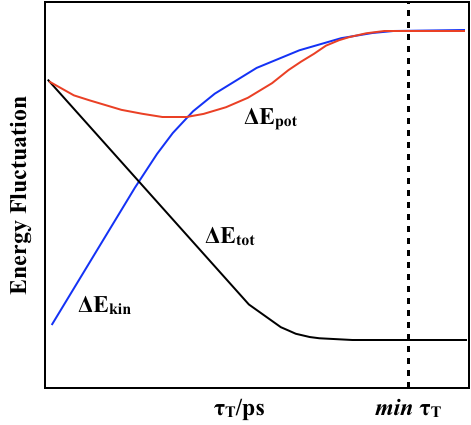
\includegraphics[width=0.35\textwidth]{gfx/image25.png}
\caption{Schematic illustration of the variation of energy (total, kinetic and potential) as a function of thermostat constant. The recommend values are those ${\tau}_{ T}{\geq}$ \textit{min${\tau}$}$_{T}$}
\label{fig:5b}
\end{figure}

\subsection{Thermostat and Barostat}
\label{sec:thermostat}
For any ensemble employed (barring the microcanonical) it is necessary to use
a \textit{thermostat} to fix the temperature and/or a \textit{barostat} to fix
the pressure. In general terms, these constrains ($T$, $P$) are
obtained modifying the Hamiltonian expressions of movement by adding an
artificial coupling. The commonly used thermo/barostats are those proposed by
Nos\'{e} and later modified by Hoover, the Nos\'{e}-Hoover \citep{hoover1985},
however there is a trend to employ more advanced propositions such as
those by Martyna-Tobias-Klein \citep{martyna1992} who use a series of
Nos\'{e}\textendash{}Hoover thermostats to construct
a Nos\'{e}\textendash{}Hoover "chain".  The choice of coupling is critical to
the outcome of the simulation \citep{shirts2013}
and an inappropriate use can give rise to results which are biased
or even unphysical \citep{wong2016}, \textit{e.g}. the use of
the Berendsen thermostat \citep{berendsen1984},
once popular, is now generally discouraged.

The strength or magnitude of the coupling is expressed in terms of the
thermostat or barostat constant, {${\tau}$}, which is usually given in time
units. In order to define the appropriate value of the thermostat or barostat
constant, one can run several MS with different values of {${\uptau}$} aiming
at ensuring that the total, kinetic, and potential energy reach a stationary
value.

A schematic illustration is given in Fig. \ref{fig:5b}, where it is seen how a thermostat
constant of ${\tau}_{T}$ larger than \textit{min ${\tau}$}$_{T}$ assures
a stable simulation, while smaller values provide for unphysical fluctuations.
Unreassuringly, the value of the thermostat/barostat constant is an extensive quantity and a function of
the particular system and the best advice is to select this value by using this
simple test. As a guideline reference one may use values of {${\uptau}$} of 0.5 to 2 ps
(Nos\'{e}-Hoover) for the case of the thermostat, and 0.2 to 1 ps (Nos\'{e}-Hoover) for the case of the barostat. There are no particular special
considerations to be taken into account in terms of the thermo/barostats for
interfacial systems, hence general suggestions applicable to bulk MS uphold. For an excellent
discussion concerning thermostats and barostats, the reader is referred to the
textbook by Tuckerman \citep{tuckerman2010}.


\subsection{Force Fields}
\label{sec:forcefields}
In MS, the force field follows from the description of the molecule and defines
its interactions with other molecules. In classical atomistic simulations,
there are three different levels of detail used to describe a molecule: all
atoms (AA), whereas the name implies, all individual atoms are represented by
centers of force; united atoms (UA), where the hydrogen atoms are included in
the representation of the associated heavier atoms and coarse-grained (CG)
representations, where larger groups of atoms, typically incorporating three to
four heavy atoms and their associated hydrogens are represented in a single
bead. Fig. \ref{fig:9b} displays models for n-decane (n-C$_{10}$H$_{22}$) for all three strategies.

\begin{figure}
	\centering
	\begin{subfigure}{0.27\textwidth} % width of left subfigure
    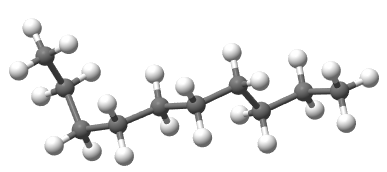
\includegraphics[width=1\textwidth]{gfx/image26.png}
		\caption{All Atoms (AA)} % subcaption
	\end{subfigure}
	\begin{subfigure}{0.27\textwidth} % width of left subfigure
    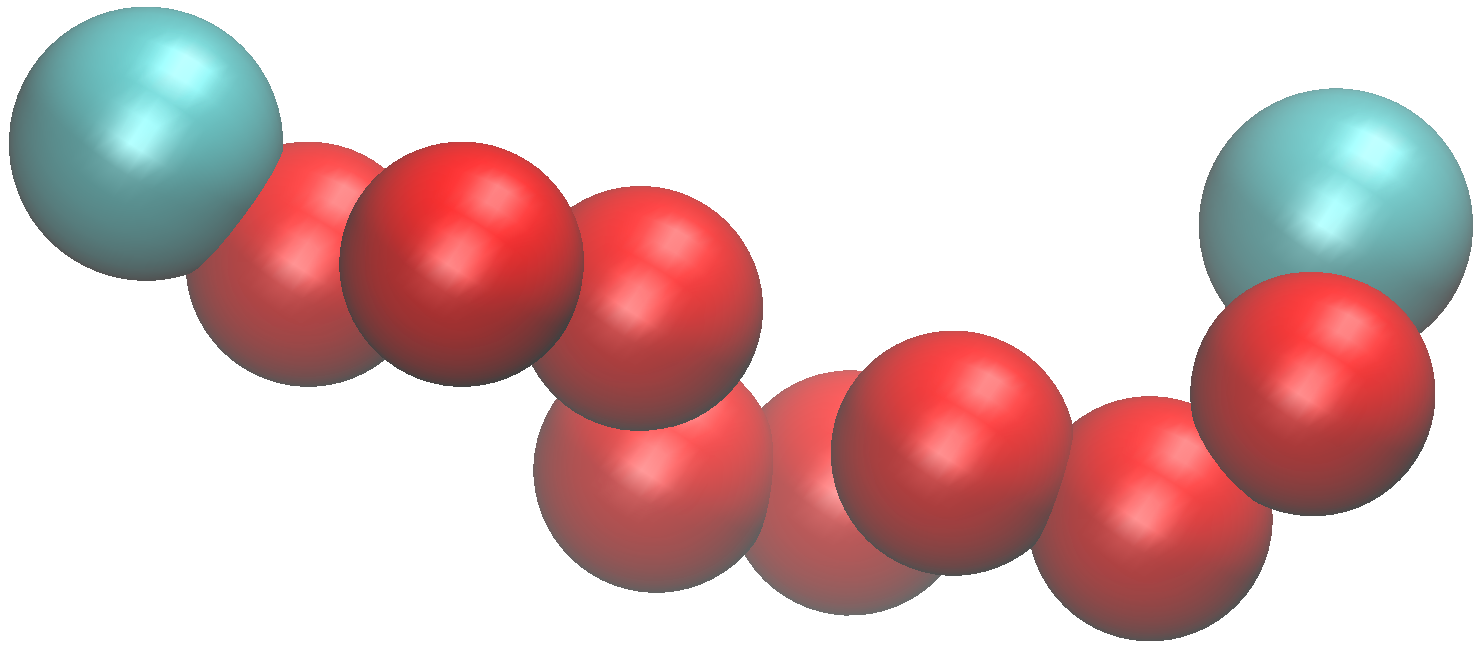
\includegraphics[width=1\textwidth]{gfx/image27-tiff.png}
		\caption{United Atoms (UA)} % subcaption
	\end{subfigure}
	\begin{subfigure}{0.27\textwidth} % width of left subfigure
    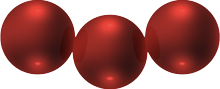
\includegraphics[width=1\textwidth]{gfx/image28.png}
		\caption{Coarse-grained atoms (CG)} % subcaption
	\end{subfigure}
  \caption{Plausible molecular descriptions for n-C$_{10}$H$_{22}$}
  \label{fig:9b}
\end{figure}

One can see from Fig. \ref{fig:9b} that it is necessary to track a total 32 particles (and possibly
an equal number of partial charges) in an AA description; 10 particles in the
UA description and only 3 in a CG description of n-C$_{10}$H$_{22}$.
Considering that the interaction between two single molecules at close range
involves the calculation of the square of these interactions, it is evident how
rapidly the use of UA and CG models imply orders of magnitude speedup in
the MS, as more than 90\% of the time in a MS code is spent in the evaluation
of the force fields. The crux of the matter is not to lose accuracy for the
sake of computational efficiency. The selection of the level of description
depends on the properties of interest, but thankfully for the case of
interfacial properties, UA and even CG seem more than adequate
\footnote{See for example the results of the 9$^{\mathrm{th}}$
Industrial Fluid Properties Simulation Challenge
(\url{http://fluidproperties.org}) where a blind test of the capabilities of
diverse force fields was performed by predicting the interfacial tension of
oil/water systems at high temperatures and pressures. Coarse Grained models
\citep{herdes2018} fared as well as more detailed UA and AA models\citep{chen2018}.
See also Ref. \citep{avendano2011} for an example relevant to this manuscript.}.
In many cases for
simple fluids, the reduction in the fidelity of the model does not have an
influence on the accuracy of the results. 
Some detail is obviously lost upon coarse-graining,
which might be relevant if the onus is on exploring the interfacial orientation
and /or charged fluids. In these cases, the use of UA models seems an
acceptable compromise. 

\begin{table}
\begin{mdframed}[linewidth=0pt,backgroundcolor=LiveCoMSLightBlue!8,fontcolor=LiveCoMSDarkBlue!80!black]
  \caption{Contribution to the potential energy in the TraPPE UA for n-C$_{10}$H$_{22}$. $k_B$ is Boltzmann’s constant. $\theta$ is the bond angle between three consecutive united-atoms, and subscript $_0$ denotes its equilibrium value. $\phi$ is the dihedral angle between four consecutive united- atoms. $r_{ij}$ is the distance between united-atoms i and j. $\epsilon_{ij}$ is the energy parameter of the interaction, whereas $\sigma_{ij}$ is the Lennard-Jones size parameter.}
  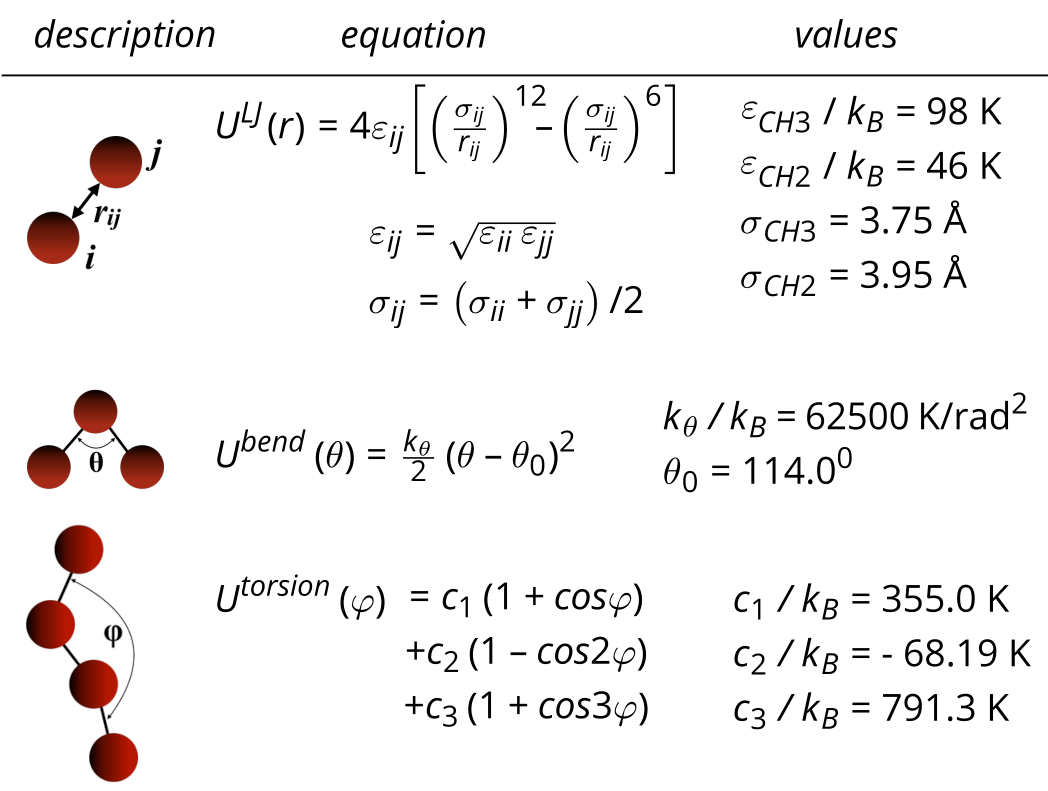
\includegraphics[width=\linewidth]{gfx/graphics-table-2.png}
%\begin{tabularx}{\textwidth}{
%p{\dimexpr 0.18\linewidth-2\tabcolsep}
%p{\dimexpr 0.43\linewidth-2\tabcolsep}
%p{\dimexpr 0.40\linewidth-2\tabcolsep}}
%\centering\arraybackslash{}\textit{description} & \centering\arraybackslash{}\textit{equation} & \centering\arraybackslash{}$values$ \\
%\midrule
%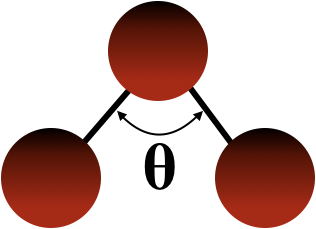
\includegraphics[width=\linewidth]{gfx/image30.png} & $U^{bend}\left(\theta\right)=\frac{k_{\theta}}{2}\left(\theta-\theta_{0}\right)^{2}$ & $k_{{\theta}}/ k_{B}$ = 62500 K/rad$^{2}$ \par ${\theta}_{0}$ = 114.0$^{0}$ \\
%
%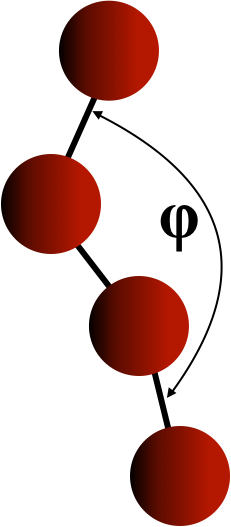
\includegraphics[width=\linewidth]{gfx/image32-2.png}\vspace{-20pt} & 
%$U^{torsion}\left(\varphi\right)$
%$\begin{array}{cc}
% & = c_{1}\left(1+cos\varphi\right)\\
% & + c_{2}\left(1-cos2\varphi\right)\\
% & + c_{3}\left(1+cos3\varphi\right)
%\end{array}$
%                       & $c_{1}/ k_{B}$ = 355.0 K \par $c_{2}/ k_{B}$ = - 68.19 K \par $c_{3}/ k_{B}$ = 791.3 K. \\
%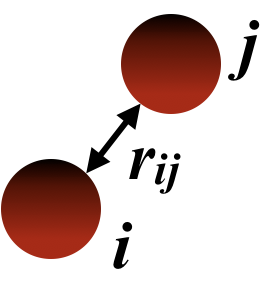
\includegraphics[width=\linewidth]{gfx/image34.png} & \vspace{-20pt} 
%$U^{LJ}\left(r\right)$
%$\begin{array}{cc}
%  &=4\varepsilon_{ij}\left[\left(\frac{\sigma_{ij}}{r_{ij}}\right)^{12}-\left(\frac{\sigma_{ij}}{r_{ij}}\right)^{6}\right] \\
%  &\varepsilon_{ij}=\sqrt{\varepsilon_{ii}\,\varepsilon_{jj}} \\
%  &\sigma_{ij}=\left(\sigma_{ii}+\sigma_{jj}\right)/2
%\end{array}$
%                  & ${\varepsilon}_{CH3}$ / $k_{B}$ = 98 K \par ${\varepsilon}_{CH2}$ / $k_{B}$ = 46 K \par ${\sigma}_{CH3}$ = 3.75 \AA{}  \par ${\sigma}_{CH2}$ = 3.95 \AA{} \\
%\end{tabularx}
\end{mdframed}
\end{table}

\begin{mdframed}[linewidth=0pt,backgroundcolor=LiveCoMSLightBlue!8,fontcolor=LiveCoMSDarkBlue!80!black]
  \textbf{EXAMPLE 3: \textit{Selection of force field}}

The molecule description, its values, and restrictions depend on the type of
force field used. As an example, the UA force field for
n-C$_{10}$H$_{22}$ can be described by using the TraPPE-UA model (\url{http://chem-siepmann.oit.umn.edu/siepmann/trappe/index.html}).
In this case, the potential energy $U$ is given by:
\begin{equation}
U=U^{str}\left(r\right)+U^{bend}\left(\theta\right)+U^{torsion}\left(\varphi\right)+U^{LJ}\left(r\right)
\end{equation}
where $U^{str}$ is the stretch, $U^{bend}$ is the bending,
$U^{torsion}$ is the torsional and $U^{LJ}$ is the
Lennard-Jones potentials. In TraPPE-UA, the stretch contribution is described
by a rigid bond between two consecutive united-atoms with a length of 1.54
\AA{} for the case of decane. The remaining terms are summarized in Table 2.
Here $k_{B}$ is Boltzmann's constant. ${\theta}$ is the bond angle between
three consecutive united-atoms, and subscript 0 denotes its equilibrium value.
${\varphi}$ is the dihedral angle between four consecutive united- atoms.
$r_{ij}$ is the distance between united-atoms $i$ and
$j$. ${\varepsilon}_{ij}$ is the energy parameter of the interaction,
whereas ${\sigma}_{ij}$ is the Lennard- Jones size parameter. 

In the case of a CG force field, n-C$_{10}$H$_{22}$ can be represented by three
tangential spheres. Using the Mie potential (See Ref. \citep{muller2014} and
references therein), these spheres interact with each other according to:
\begin{equation}
\begin{aligned}
  U\left(r\right) &= C\varepsilon_{ij}\left[\left(\frac{\sigma_{ij}}{r_{ij}}\right)^{\lambda_{r_{ij}}}-\left(\frac{\sigma_{ij}}{r_{ij}}\right)^{\lambda_{a_{ij}}}\right] \\
  & C = \left[\frac{\lambda_{r_{ij}}}{\lambda_{r_{ij}}-\lambda_{a_{ij}}}\left(\frac{\lambda_{r_{ij}}}{\lambda_{a_{ij}}}\right)^{\frac{\lambda_{a_{ij}}}{\lambda_{r_{ij}}-\lambda_{a_{ij}}}}\right]
\end{aligned}
\end{equation}
\ignorespacesafterend
where {${\lambda}$}$_{rij}$ and {${\lambda}$}$_{aij}$ are the repulsion and
attraction parameters of the intermolecular potential, respectively.
$r_{ij}$ is the center-to-center distance of the interacting segments.
${\varepsilon}_{ij}$ is the energy scale corresponding to the potential well
depth, ${\sigma}_{ij}$ is the length scale, corresponding loosely with an
effective segment diameter. The Mie potential reverts to the well-known
Lennard-Jones model if the repulsive and attractive exponents are taken as 12
and 6, respectively. For the case of n-C$_{10}$H$_{22}$ the Mie parameters are
\citep{mejia2014a}:
{${\lambda}$}$_{rii}$ = 19.21, {${\lambda}$}$_{aii}$ = 6,
${\varepsilon}_{ii}$ / $k_{B}$ = 414.90 K and ${\sigma}_{ii}$
= 4.629 \AA{}.

For the case of heteronuclear molecules or mixtures, the cross parameters for the Mie are obtained by using the following combination rules:
\begin{align}
  \sigma_{ij} &= \left(\sigma_{ii}+\sigma_{jj}\right)/2 \\
  \varepsilon_{ij} &= \left(1-k_{ij}\right)\frac{\sqrt{\sigma_{ii}^{3}\sigma_{jj}^{3}}}{\sigma_{ij}^{3}}\sqrt{\varepsilon_{ii}\,\varepsilon_{jj}} \\
  \left(\lambda_{k_{ij}}-3\right) &= \sqrt{\left(\lambda_{k_{ii}}-3\right)\left(\lambda_{k_{jj}}-3\right)} \\
\end{align}
where $\lambda_{k_{ii}}$ = $\lambda_{r_{ii}}$ or $\lambda_{a_{ii}}$, etc., and $k_{ij}$ is a binary
interaction parameter, which can be obtained from experimental data of phase
equilibria.

In the supplementary information, the force field for the CO$_{2}$ and
n-C$_{10}$H$_{22}$ pure fluids as well as for the CO$_{2}$ + n-C$_{10}$H$_{22}$
mixture are included for both TraPPE-UA and CG-Mie schemes.
\end{mdframed}

\subsection{Cutoff radius and long range corrections} 
\label{sec:cutoff}
The most time-consuming aspect of any simulation is related to the calculation of the nonbonded (van
der Waals or long-range interactions) terms in the potential energy function.
Approximately, the number of interactions that must be calculated scale with
the square of the number of force centers (although with the use of elaborate
algorithms this may be scaled down). In order to reduce the calculation time
associated with the evaluation of these long-range interactions, a truncation
of the energy (or force) is used. In other words, the energy (or force) is set
to zero for distances larger than a given radius, traditionally called the
cutoff radius ($r_c$). One option is to cut the potential at $r_c$. Another 
option is switching the tail off smoothly, which makes the potential energy zero after
a given $r_c$. 

%\begin{figure}
%	\centering
%	\begin{subfigure}{0.2\textwidth} % width of left subfigure
%    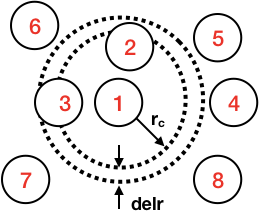
\includegraphics[width=0.45\textwidth]{gfx/image41.png}
%    \caption{
%    Lennard-Jones:
%    $U\left(r\right)=\left\{ \begin{array}{cc}
%    4\varepsilon\left[\left(\frac{\sigma}{r}\right)^{12}-\left(\frac{\sigma}{r}\right)^{6}\right] & \quad r\leq r_{cut}\\
%    0 & \quad r\geq r_{cut}
%    \end{array}\right.$
%    }
%	\end{subfigure}
%	\begin{subfigure}{0.2\textwidth} % width of left subfigure
%    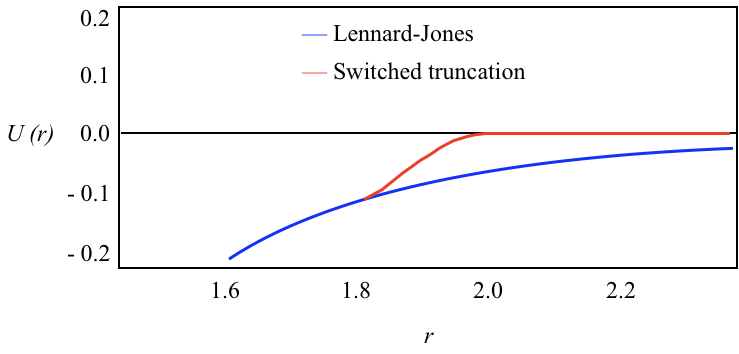
\includegraphics[width=0.45\textwidth]{gfx/image42.png}
%    \caption{
%    Lennard-Jones switched:
%    $U\left(r\right)=\left\{ \begin{array}{cc}
%    U\left(r\right)-U\left(r=r_{cut}\right) & \quad r\leq r_{cut}\\
%    0 & \quad r\geq r_{cut}
%    \end{array}\right.$
%    }
%	\end{subfigure}
%  \caption{Cutoff radius, $r_{c}$ as applied to the Lennard-Jones
%potential. (left) schematic illustration of $r_{c}$ and Verlet delta
%of $r_{c}$ (delr). (right) The long tail of the attractive potential
%tails off slowly toward the value of zero (Blue curve). Switching the tail off
%smoothly makes the potential energy zero after a given cutoff. Lower figure
%shows how the only interactions calculated for particle 1 are those with
%particles 2 and 3, rather than all the particles in the box, an aspect which
%significantly speeds up the simulation. }
%\label{fig:10}
%\end{figure}

Ideally, one would not need to consider a cutoff radius and would calculate the
interaction between all particles in the simulations cell. Many of these
interactions correspond to pairs of molecules which are at a significant
distance from each other and essentially do not interact. Fig. \ref{fig:11} shows the
effect of a cutoff radius, where the calculation of forces is only taken into
account for molecules whose centers are at a distance $r$ {\textless}
$r_{c}$ apart. Note however that the application of a cutoff is, in effect,
modifying the potential (and consequently the results) hence the balance
between the speed up of the calculation and the accuracy of the results is
important. Excellent discussions of this topic have been provided in Ref.
\citep{holcomb1993,trokhymchuk1999,mecke1997,duque2004,blas2008}

In homogeneous systems, the application of short cutoffs can be offset by
adding long range corrections (LRC) based on a mean field value. For the case
of inhomogeneous systems, clearly this must be done with attention,
particularly for molecules in the vicinity of interfacial region where
different environments are present at either side of the interface
\citep{lotfi1990,janecek2006,siperstein2002,lishchuk2018}
For most simple systems, given the
availability of cheap computer power, the recommended practice of MS of interfacial
properties is to use large cutoffs rather than to have to correct the results. In
order to define its value, it is advised to run a few simulations to define the
lower value to capture the interfacial properties. As an example, Fig. \ref{fig:11}
typifies the impact of cutoff in bulk and interfacial properties. 

\begin{figure}
  \centering
%  \begin{subfigure}{0.4\textwidth} % width of left subfigure
%    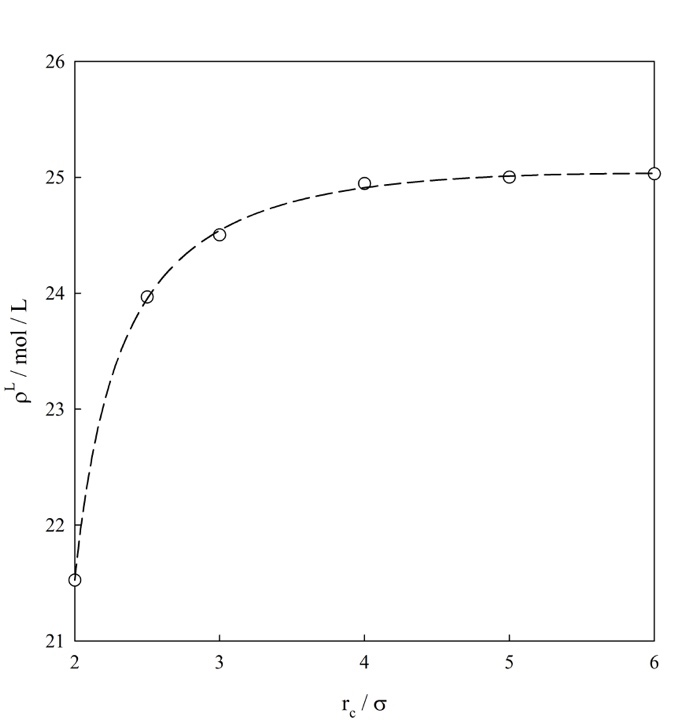
\includegraphics[width=1\textwidth]{gfx/image45.jpeg}
%	\end{subfigure}
%  \begin{subfigure}{0.4\textwidth} % width of left subfigure
%    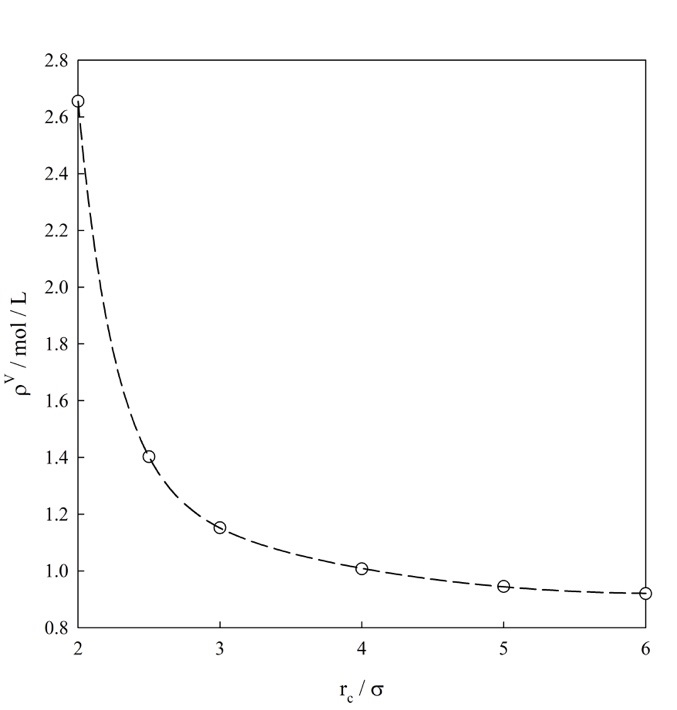
\includegraphics[width=1\textwidth]{gfx/image46.jpeg}
%	\end{subfigure}
%  \begin{subfigure}{0.4\textwidth} % width of left subfigure
%    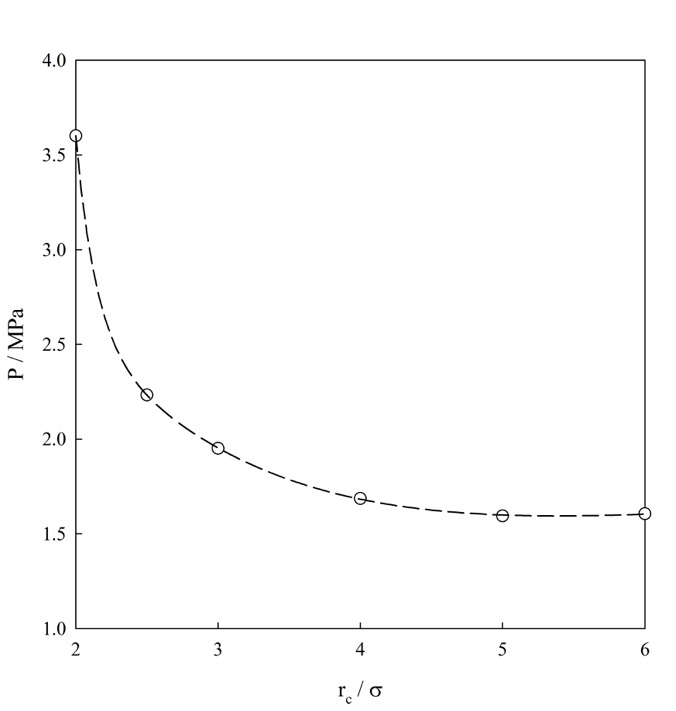
\includegraphics[width=1\textwidth]{gfx/image47.jpeg}
%	\end{subfigure}
%  \begin{subfigure}{0.4\textwidth} % width of left subfigure
%    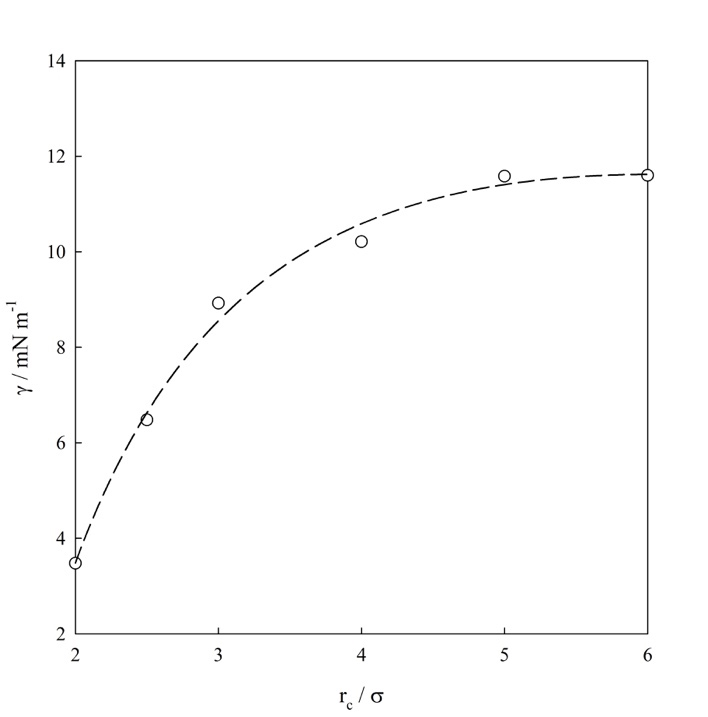
\includegraphics[width=1\textwidth]{gfx/image48.jpeg}
%	\end{subfigure}
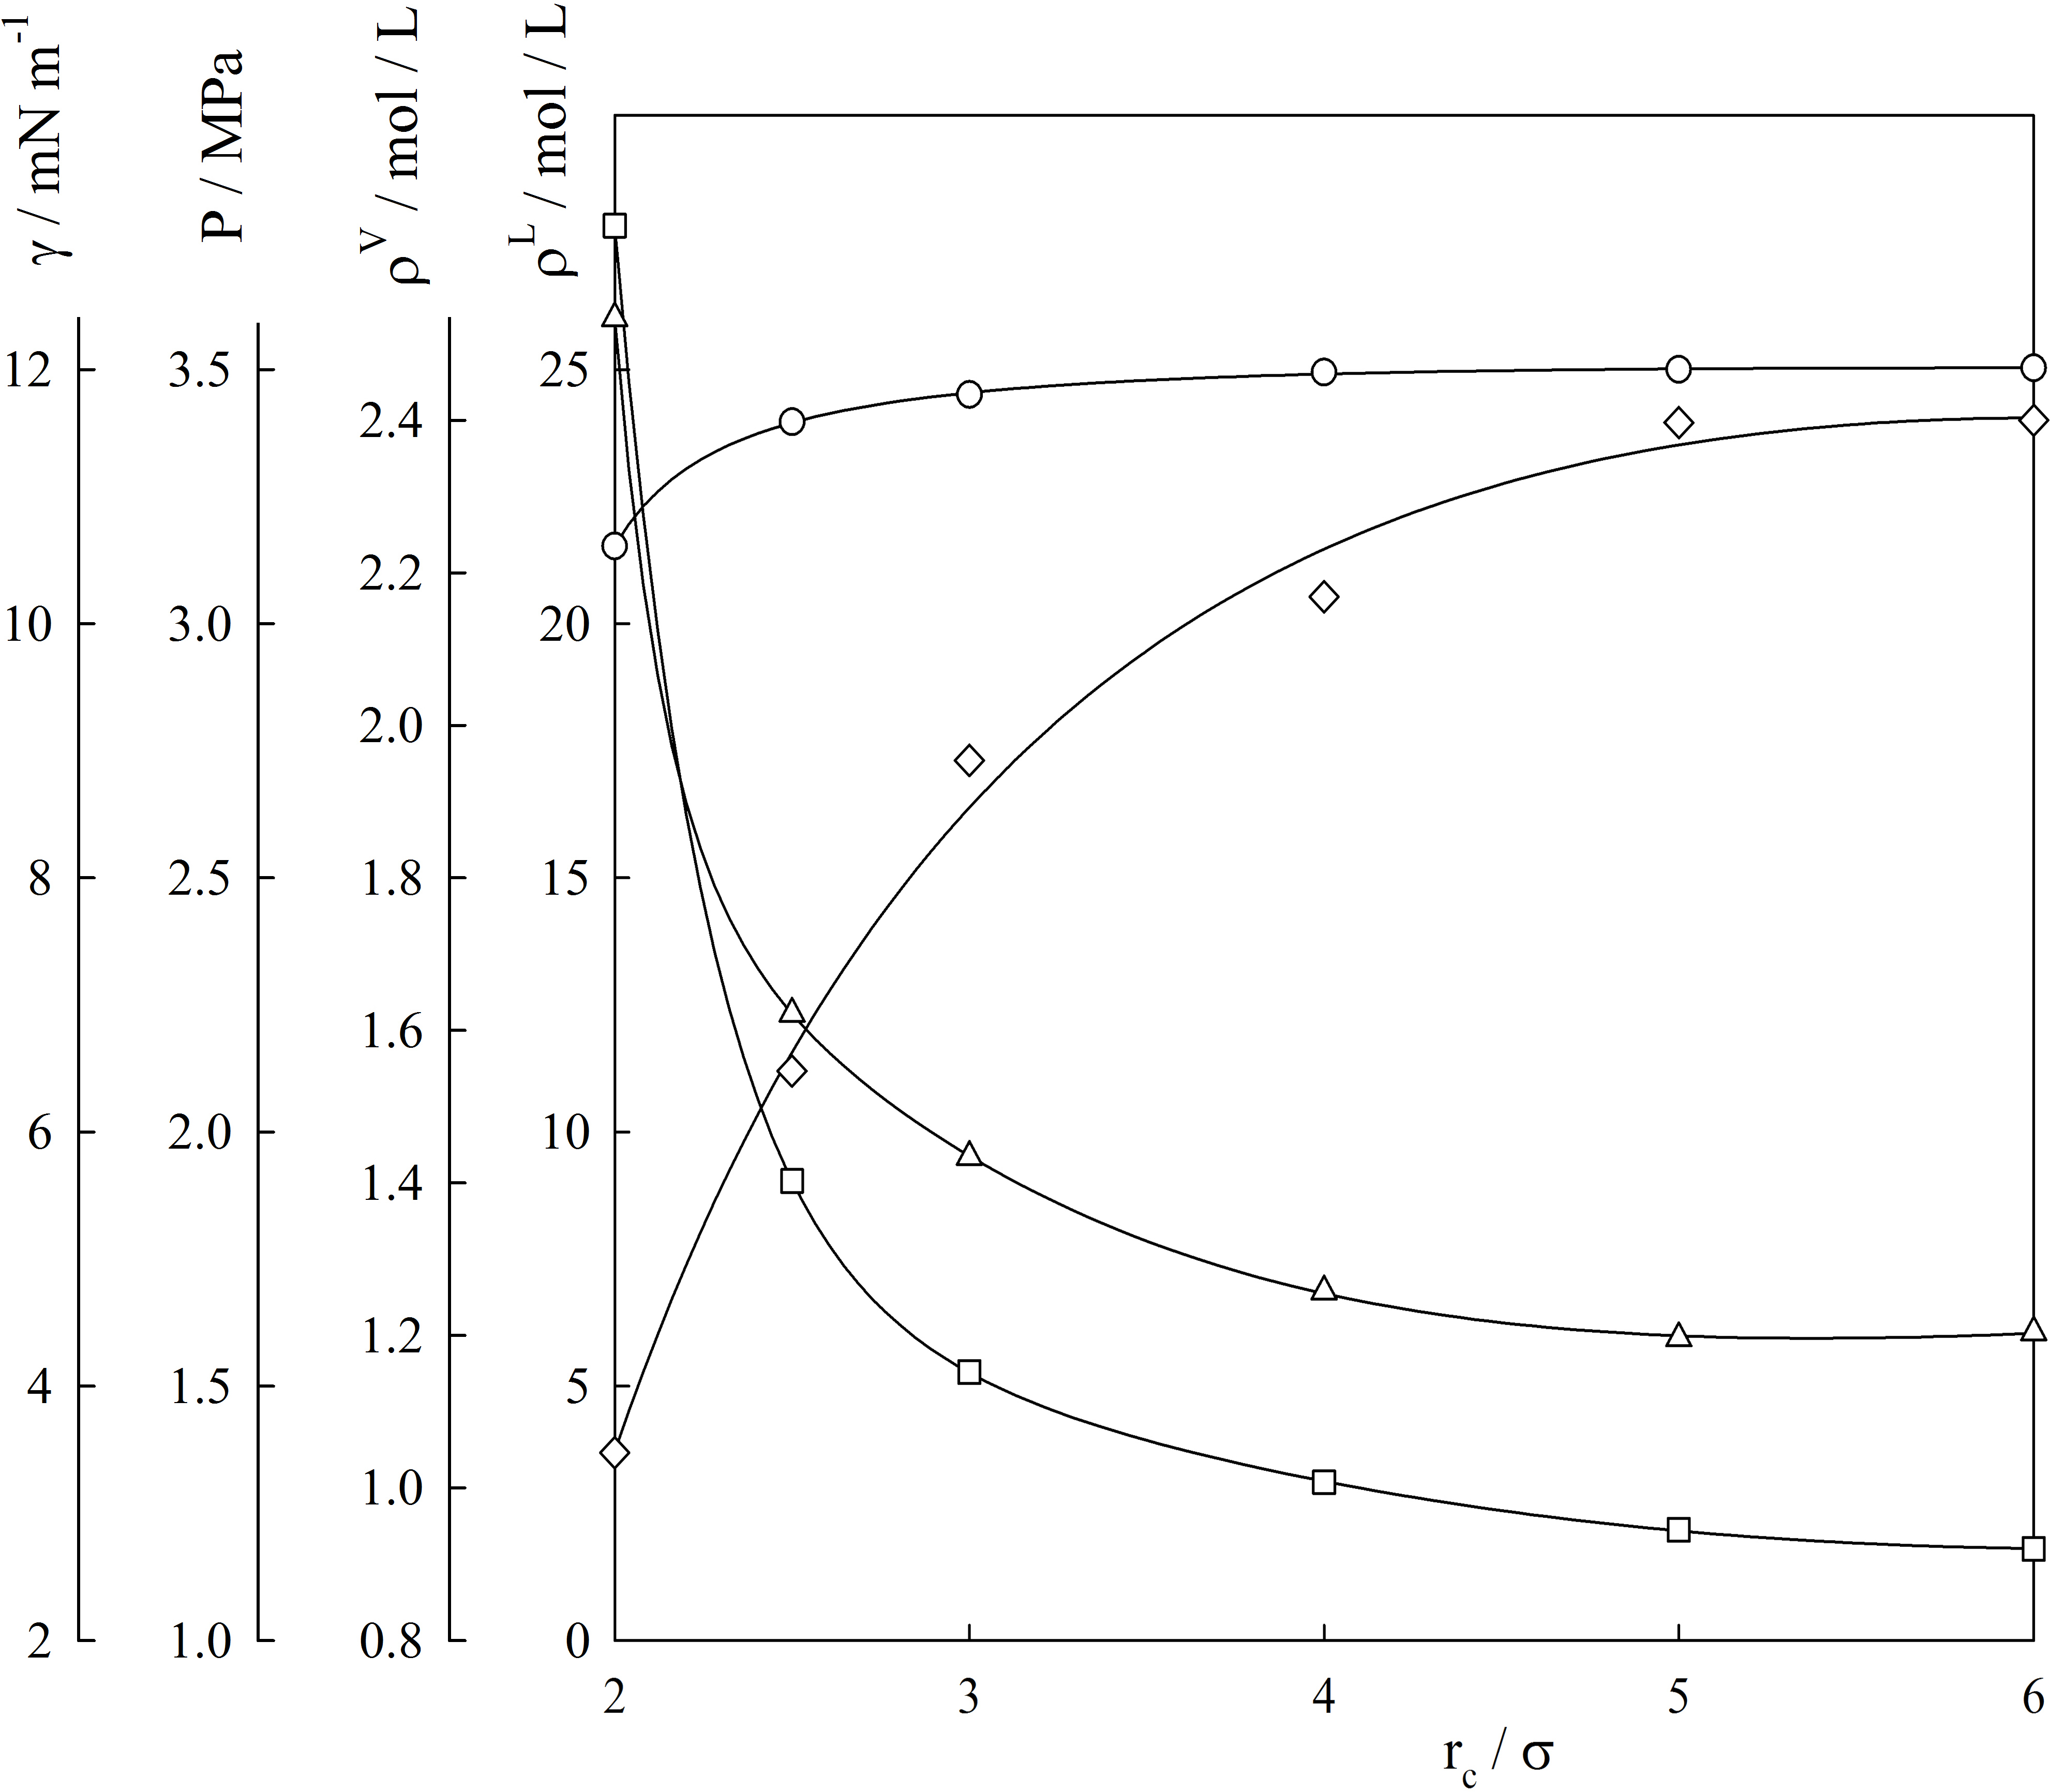
\includegraphics[width=\linewidth]{gfx/fig_11_op4.JPG}
\caption{Impact of cutoff ($r_{c}$) on the bulk and interfacial properties for the case of CO$_{2}$ (single Mie sphere) at 240 K. $\lozenge$, surface tension $\gamma$; $\triangle$, vapor pressure $P$; $\ocircle$, liquid density $\rho^L$; $\square$, vapor density $\rho^V$.}
\label{fig:11}
\end{figure}

From this figure, it is seen how at larger $r_{c}$ all properties of
relevance reach a stationary value. Clearly, the large cutoff can never be more
than half of the smallest cell dimension (e.g., $L_{x}$/2).
Therefore, as a suggestion, a value of cutoff equal or larger than
6 ${\sigma}_{\mathrm{max}}$ (typically $\approx 2$ nm) will be an adequate choice to avoid the
truncation and system size effects involved in the phase equilibrium and
interfacial properties calculations.

For the case of fluids with electrostatic contributions to the energy, the
potential energy decays proportional to $r^{2}$ (rather than
$r^{6}$ as in the case of simple dispersion).
In this case, the definition of "a short distance $r_{c}$ where the
potential tails to effectively a zero value", ceases to make sense, as
illustrated in Fig. \ref{fig:6}. 

\begin{figure}
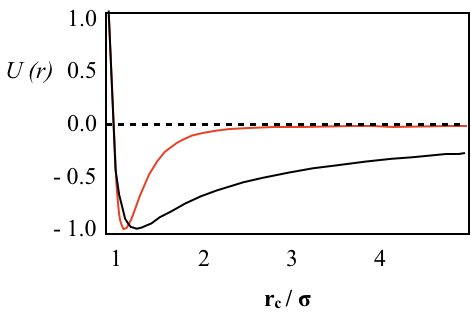
\includegraphics[width=0.5\textwidth]{gfx/image49.png}
\caption{Energy potential for fluids with and without electrostatic contribution to the energy. (\textcolor{color-3}{\textemdash}) Lennard -- Jones; (\textemdash) Coulomb}
\label{fig:6}
\end{figure}

The na\"{i}ve solution suggests using a simulation cell with very long
dimension $L_{x}$ ($r_{c},_{max}$ = $L_{x}$/2).
Unfortunately, such large $L_{x}$ implicates a very (very) big
simulation box, both impractical and ultimately unnecessary. This issue can
be solved by using a numerical strategy that converts the real space to
the reciprocal (or complex) space effectively providing for an alternative force
calculation.  The most popular of said methods, Ewald summation \citep{ewald1921},
proposes to neutralize
each partial charge in the fluid by a superposition of spherical Gaussian
distributions of opposite charge while employing a second Gaussian of similar
charge to the original to annul the effect of the first set. The resulting
potential stemming from these Gaussians is obtained from Poisson's equation and
is solved as a Fourier series. This combination provides a route to replace the
real space (where $r_{c}$ would be very large) to a combination of
real, and reciprocal (or complex) space. In practice, Ewald's methodology
is controlled by three variables: the real space cutoff ($r_{c}$); the
convergence parameter and the largest reciprocal space vector used in the
reciprocal space sum. The convergence parameter and reciprocal space vector are
obtained using a minimization procedure, which uses the Coulombic energy and
the Coulombic virial. From a technical view point, a very efficient algorithm
for optimization is implemented in DL\_POLY software, where these parameters are
obtained when the simulation starts. Ewald summations are time consuming from
a point of view of the MS so efforts to reduce the simulation time are in
continuous development (e.g. reaction field \citep{barker1973,watts1974},
the smoothed particle mesh \citep{darden1993},
and the Wolf \citep{wolf1999} methods; see further details in Ref. \citep{allen2017}).
While the electrostatic potentials are the
prototypical examples of long-ranged potentials, some very soft potentials
( \textit{e.g.,} an 8-6 Mie ) will also exhibit relatively long attractive
tails, for which Ewald summations can also be applied in order to avoid the use
of calculating long range corrections \citep{kissel}.

\subsection{Simulation length} 
\label{sec:length}
Simulations are divided into two stages: equilibration and production. During
the equilibration, the thermostat and/or barostat force the system to reach the
desired thermodynamic state conditions. In the subsequent production stage, the
thermostat and/or barostat are commonly (although not necessarily) turned off,
and the system naturally evolves in $NVE$ ensemble, where statistics are
collected. As a rule of thumb, the production length is at least twice the
equilibration stage. 

In the case of MS based on MD, the simulation length is usually defined in
terms of the requested time or the total number of steps using a defined time
step. The specification of the time step is a function of the stability of the
numerical algorithm used to integrate the Newtonian equations. In the case of
MD for interfacial properties, the Verlet leapfrog algorithm is commonly used
with a time step from 0.003 to 0.01 ps. As a reference, the order of magnitude 
of the time step, $\Delta t$, can be estimated from the following equation
for Lennard-Jones fluids:
\begin{equation}
\Delta t=0.01\sqrt{\frac{m\:\sigma^{2}}{\varepsilon}}
\end{equation}
where $m$, $\varepsilon$, and $\sigma$  take their usual meaning (as
in the LJ potential). For the particular case of interfacial properties of pure
fluids, simulations are typically longer than those of one phase bulk fluids,
namely because of the requirement of the establishment of the interface and the
relatively slow diffusion of components through the otherwise large systems.
For pure components, 10 to 15 ns for the equilibration stage, and 30 ns for the
production state are common times. For the case of mixtures, a longer
equilibrations are needed, to the tone of 70 to 80 ns after which production
runs should be set for at least another 150 ns.

In the case of MC simulations, the simulation length is usually defined in
terms of the number of cycles, where each cycle consists of $N$ randomly
selected moves that include translation, rotation, flips, etc. A typical MC run
in the $NVT$ or $NP_{zz}AT$ ensemble consists of
$O$(10$^{6}$) cycles for equilibration and $O$(10$^{7}$) cycles
for production.

\section{Post-processing}
\label{sec:post-proc}
Interfacial tensions and associated properties are rarely calculated
on-the-fly, but rather obtained from post-processing the results of a MS. This
section is devoted to describing the calculation of the interfacial density,
concentration profiles and the interfacial tension. Additionally, the evaluation
of other derived
properties, such as isothermal Gibbs adsorption and surface entropy and surface
enthalpy are illustrated. 

\subsection{Calculation of interfacial density profiles and related interfacial properties}

The density profile is calculated by dividing the simulation box
($L_{x}L_{y}L_{z}$) in $n$ slabs
($n{\simeq}$ 250 to 500) along the $z$ direction, as it is
illustrated in Fig. \ref{fig:7}. At each position, the density of a molecule
$i$ in the slab $j$, {${\rho}$}$_{i}$  is calculated as:
\begin{equation}
\rho_{i}=\frac{\left\langle N_{i}\right\rangle }{V_{j}}=\frac{\left(\sum_{s=1}^{ns}N_{is}\right)/ns}{V_{j}}
\end{equation}
where $N_{i}$ is the number of molecules $i$ in the $j$
slab; $s$ represents the sites of the molecule $i$, and
$ns$ is the number of sites per molecule. $V_{j}$ is the volume of each
slab, which is $L_{x}L_{y}L_{z\,j}$. As an
example, the density of n-C$_{10}$H$_{22}$ in the slab $j$ can be
calculated as {${\rho}$}$_{i}^{\mathrm{C10H22}}$
= (($N_{i}^{\mathrm{CH3}}$
+ $N_{i}^{\mathrm{CH2}}$)/10)/$V_{j}$ for the case of UA
whereas {${\rho}$}$_{i}^{\mathrm{C10H22}}$
= ($N_{i}$/3)/$V_{j}$ for the case of CG model.
Note that we suggest to calculate the densities based on the number of sites observed
in a given slab. In most cases of chain fluids, molecules will span several slabs,
and this must be accounted for.

\begin{figure}
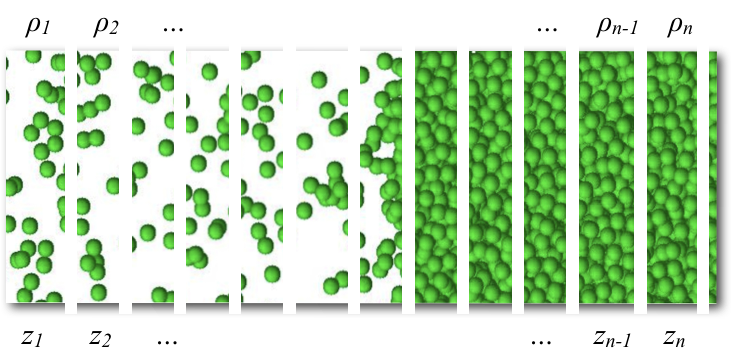
\includegraphics[width=0.5\textwidth]{gfx/image51.png}
\caption{Partitioning of the simulation box in $n$ vertical slabs for computing the density profile, ${\rho}_{\mathrm{i}}$.}
\label{fig:7}
\end{figure}

In order to guarantee that the simulated systems are at a true equilibrium
state, neither transient nor steady state, it is advised to monitor the time
evolution of the concentration of species in the direction normal to the
interface, {${\rho}$}$_{i}$($z$). Holcomb \textit{et al.} \citep{holcomb1993} demonstrated that the time evaluation of
{${\rho}$}$_{i}$($z$) can bring not only a picture of the progression to
equilibrium but also provides a way to establish a true equilibrium condition.
Fig. \ref{fig:8} shows the time evolution of $z$ \textendash{} {${\rho}$}(z)
for the case of CO$_{2}$ represented as single Mie sphere (see Ref. \citep{mejia2005} for the case of
Lennard \textendash{} Jones fluid.) 

\begin{figure}
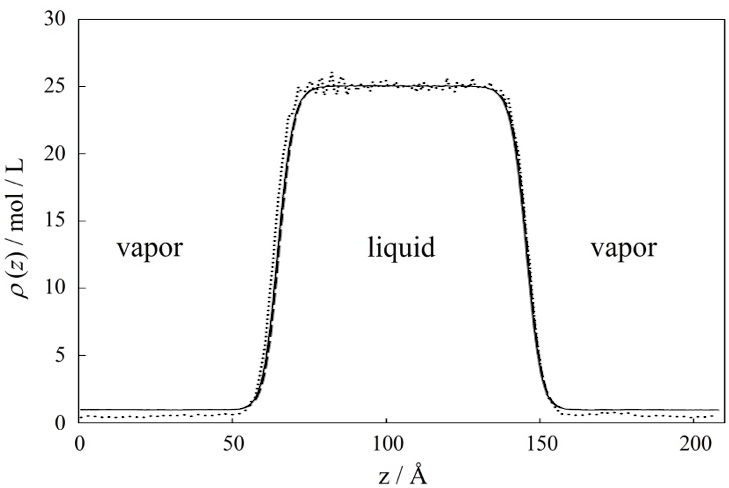
\includegraphics[width=0.5\textwidth]{gfx/Fig_14_2.jpeg}
\caption{Time evolution of {${\rho}$} vs $z$ profiles for the case of CO$_{2}$ (single Mie sphere) at 240 K at vapor \textendash{} liquid equilibria. ({\textbullet}{\textbullet}{\textbullet}) 18 ns, (${-}{-}$) 36 ns, and (\textemdash) 54 ns.}
\label{fig:8}
\end{figure}

From this figure, we can observe that as the simulation time increases, the
density in the bulk regions plateau while the interfacial regions adjust their
shape until eventually reaching a steady state ( after 36 ns in the example in
Fig. \ref{fig:8}). 

It is possible that systematic round-off errors in the simulation induce a drift
in the position of the slabs. If this is not corrected or accounted for, the
density profiles might be smeared out and interfacial widths misrepresented.
A trick of the trade is to re-center the center of mass of the system every
once in a while, or to periodically zero out the total momentum of the system,
to avoid these spurious effects.

The interfacial profiles for pure fluids and also for fluid in mixtures without
surface activity can be fitted using Eq. \ref{eq:3} which can also be used directly to
provide an estimate of the interfacial thickness. For the case of mixtures, the
interfacial concentration of species, $z$ \textendash{}
{${\rho}$}$_{i}$(z) provide a route to evaluate the surface activity of the
fluids in mixture. As an illustration, Fig. \ref{fig:9} displays the $z{-}$
${\rho}_{i}$ projections for the case of CO$_{2}$ + n-C$_{10}$H$_{22}$
mixture at 344.15 K. In this figure, we only include one vapor${-}$liquid
interface, as the system is symmetrical along the z coordinate (see Fig. \ref{fig:8}). 

\begin{figure}
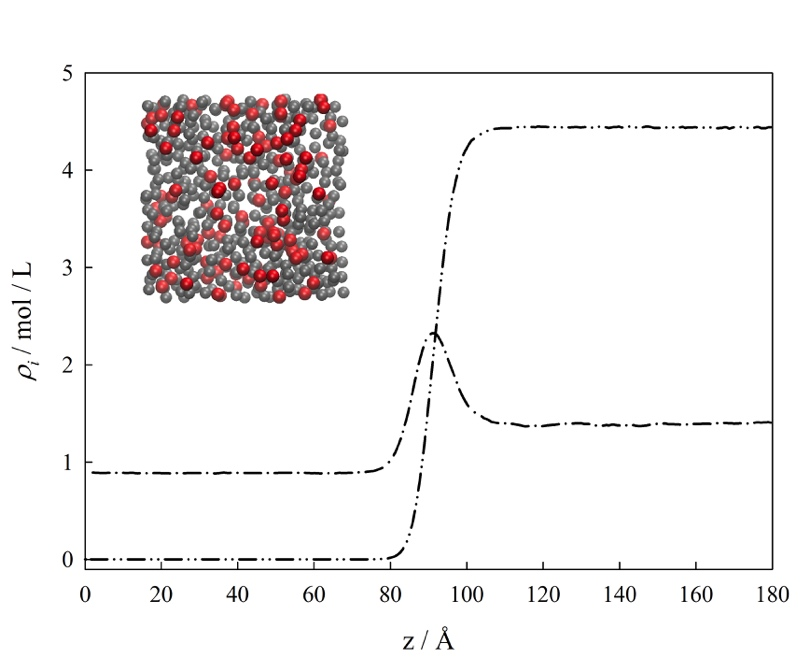
\includegraphics[width=0.5\textwidth]{gfx/image54.jpeg}
\caption{Interfacial profiles for CO$_{2}$ + n-C$_{10}$H$_{22}$ mixture at 344.15 K and P = 2.39 MPa ($x_{1}$ = 0.238). MD results for ${-}$.${-}$, $z$ \textendash{} ${\rho}_{1}$; ${-}$..${-}$, z\textendash{} ${\rho}_{2}$. Insert is a snapshot of the interfacial region, seen from the CO$_{2}$-rich side, depicting only the first layer of adsorbed molecules. CO$_{2}$ (red), n-C$_{10}$H$_{22}$ (gray).(adapted from Ref. \citep{mejia2014a})}
\label{fig:9}
\end{figure}

The interfacial profiles provide a method to evaluate the surface activity of
the fluids inside the interfacial zone. In the example of Fig. \ref{fig:9}, a positive
surface activity is seen for CO$_{2}$ (d${\uprho}_{1}$/dz = 0;
d$^{2}{\uprho}_{1}$/dz$^{2}$ {\textless} 0 in the interfacial region),
whereas n-C$_{10}$H$_{22}$ does not show surface activity. Additionally, the
interfacial density profiles provide the needed information to describe the
observed surface activity behavior in terms of the relative Gibbs adsorption
isotherm of CO$_{2}$ (1) with respect to n- C$_{10}$H$_{22}$ (2),
${\Gamma}_{12}$ (see Eq. \ref{eq:4}). Again, as an example, for the system and
condition of the figure, ${\Gamma}_{12}$ = 1.523 x 10$^{-9}$
kmol/m$^{2}$\citep{mejia2014a}.

\subsection{The mechanical route for the interfacial tension: The pressure tensor method}

The pressure tensor method is the most common way of calculating the
interfacial tension for pure fluids and fluid mixtures. The
basis of this method is to calculate the components of the diagonal element of
the inhomogeneous pressure tensor, ($P_{xx}$($z$),
$P_{yy}$($z$), $P_{zz}$($z$)) by using the
Irving-Kirkwood (IK) \citep{irving1950}
(or alternatively the Harasima \citep{harasima1957})\footnote{For
a concise discussion on the strategies of calculating the pressure tensor,
including the IK and Harasima definitions, the reader is referred to Ref. \citep{long2013}.
}
formulation which
then feeds into Eq. \ref{eq:hulshof} to be employed to calculate the tension. 

In the IK method, the pressure tensor element, $P_{kk}$ ($z$) is given by the following expression:
\begin{equation}
P_{kk}\left(z\right)=k_{B}T\rho\left(z\right)+\frac{1}{A}\left\langle \sum_{{\scriptstyle i}}^{{\scriptstyle N-1}}\sum_{{\scriptstyle j>i}}^{N}\frac{1}{\left|z_{i}-z_{j}\right|}\left(f_{ij}\right)_{k}\left(r_{ij}\right)_{k}\right\rangle 
  \label{eq:10}
\end{equation}
In Eq. \ref{eq:10}, the subscript $kk$ represents the spatial coordinate, either
$x$ , $y$, or $z$ , $k_{B}$ is Boltzmann's
constant, $T$ is the absolute temperature, $A$ is the interfacial
area, $N$ is the number of molecules, and the double sum involves the
force on molecule $i$ due to molecule $j$. $f_{ij}$ is
the force on molecule $i$ due to molecule $j$, and
$r_{ij}$ represents the distance between molecules $i$ and
$j$. It is important to note that Eq. \ref{eq:10} sums two terms.
The first term takes into account the kinetic contribution, which is
proportional to the ideal-gas pressure, while the second term corresponds to
the configurational contribution which is evaluated as \textit{ensemble averages}, as
indicated by the ${\langle}${\ldots}${\rangle}$ brackets, and not instantaneous
values.

In MD codes, the most common implementation of the algorithm is to evaluate the
average of the elements ${\langle}P_{kk}{\rangle}$ over the \textit{whole
volume} of the simulation box. Speculating over the possible reason for this
implementation of ${\langle}P_{kk}{\rangle}$ is the inspiration on
the pressure calculation in homogeneous systems, where the pressure of the
system is given by the arithmetic average of the diagonal elements: $P$
= (${\langle}P_{xx}{\rangle}$
+ ${\langle}P_{yy}{\rangle}$
+ ${\langle}P_{zz}{\rangle}$)/3, (\textit{i.e.} the trace divided by 3). As an illustration of the
underlying issue, Fig. \ref{fig:16} displays the diagonal elements of the pressure
tensor ${\langle}P_{xx}{\rangle}$,
${\langle}P_{yy}{\rangle}$, and
${\langle}P_{zz}{\rangle}$ evaluated for the whole volume of
a simulation box in an inhomogeneous system during the production stage, where
it is possible to observe that this implementation produces artificial
fluctuations in the results.  The values of
${\langle}P_{xx}{\rangle}$ and
${\langle}P_{yy}{\rangle}$ vary only along the z coordinate,
whereas ${\langle}P_{zz}{\rangle}$ should be constant along
$z$,  implies that the normal pressure ( that of the bulk phases) is
$P_{N}$ = ${\langle}P_{zz}{\rangle}$ while the tangential
components will be equal ( due to the symmetry of the problem)
$P_{T}$ = ${\langle}P_{xx}{\rangle}$
= ${\langle}P_{yy}{\rangle}$. 


\begin{figure}
	\centering
	\begin{subfigure}{0.45\linewidth} % width of left subfigure
    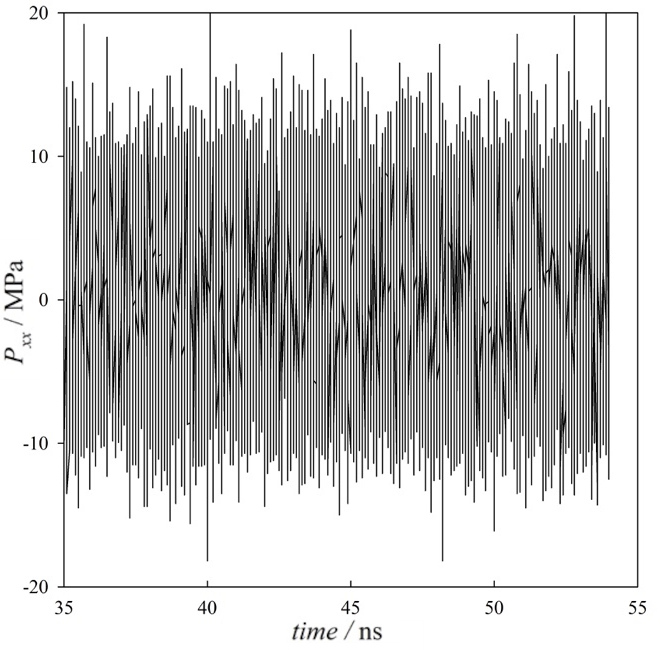
\includegraphics[width=1\textwidth]{gfx/fig_15_a.jpeg}
	\end{subfigure}
	\begin{subfigure}{0.45\linewidth} % width of left subfigure
    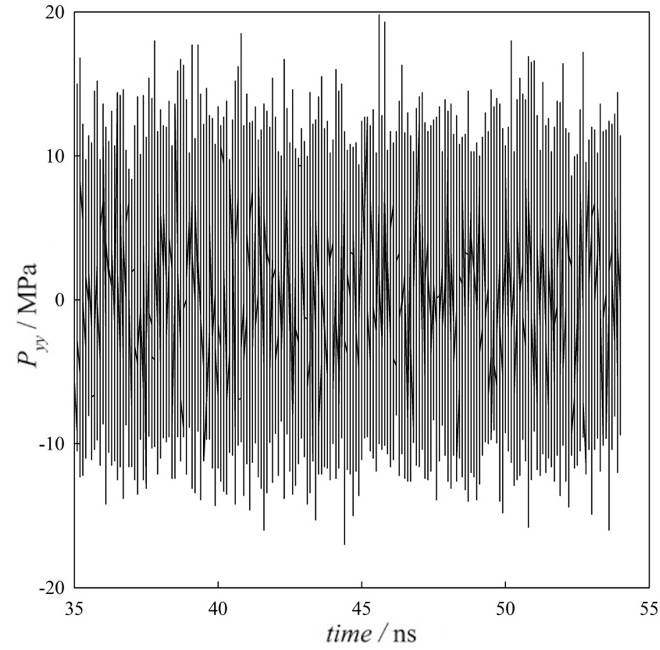
\includegraphics[width=1\textwidth]{gfx/fig_15_b.jpeg}
	\end{subfigure}
	\begin{subfigure}{0.45\linewidth} % width of left subfigure
    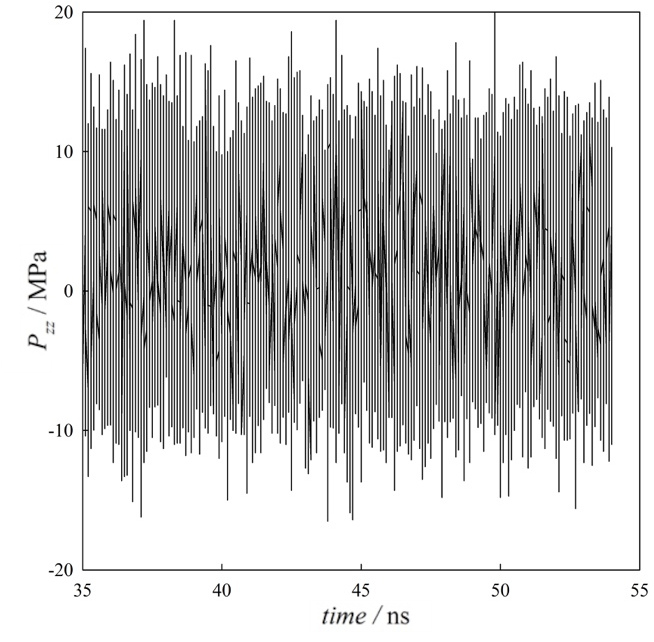
\includegraphics[width=1\textwidth]{gfx/fig_15_c.jpeg}
	\end{subfigure}
	\begin{subfigure}{0.45\linewidth} % width of left subfigure
    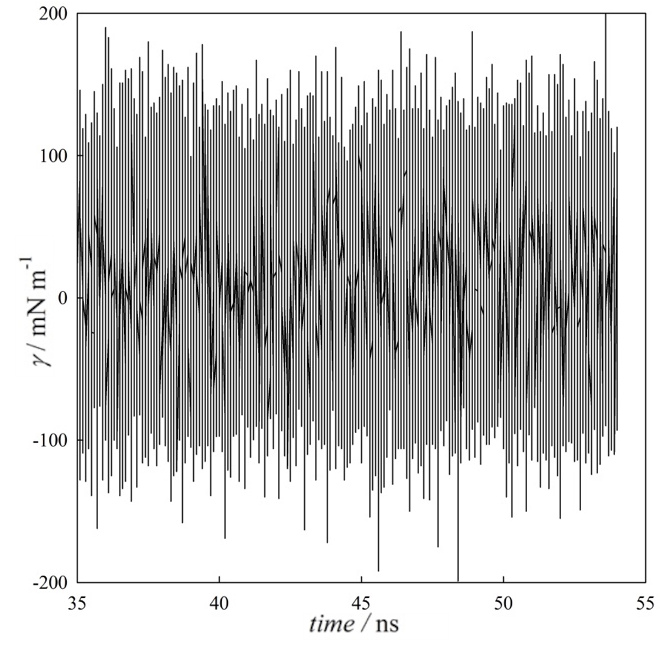
\includegraphics[width=1\textwidth]{gfx/fig_15_d.jpeg}
	\end{subfigure}
\caption{Diagonal elements of the pressure tensor ${\langle}P_{xx}{\rangle}$, ${\langle}P_{yy}{\rangle}$, and ${\langle}P_{zz}{\rangle}$ and the resulting interfacial tension, ${\gamma}$, evaluated over the volume simulation box for the case of CO$_{2}$ (single Mie sphere) at 240 K.
}
\label{fig:16}
\end{figure}

Considering the values reported in Fig. \ref{fig:16} and averaging their values
over the production stage, one obtains ${\langle}P_{xx}{\rangle}$
= 0.4072 MPa, ${\langle}P_{yy}{\rangle}$  = 0.4043 MPa, and
${\langle}P_{zz}{\rangle}$ =1.4691 MPa. Taking the average of
${\langle}P_{xx}{\rangle}$ and
${\langle}P_{yy}{\rangle}$ as $P_{T}$
= (${\langle}P_{xx}{\rangle}$
+ ${\langle}P_{yy}{\rangle}$)/2, and $P_{N}$
= ${\langle}P_{zz}{\rangle}$, Eq. \ref{eq:hulshof} can be rewritten as:

\begin{equation}
\gamma=\frac{L_{z}}{2}\left[\left\langle P_{zz}\right\rangle -\frac{\left\langle P_{zz}\right\rangle +\left\langle P_{zz}\right\rangle }{2}\right]
  \label{eq:11}
\end{equation}

In this latter equation the additional factor of 1/2, takes into account the
presence of  two interfaces in the system. Evaluating Eq. \ref{eq:11}, with
$L_{z}$ = 208 \AA{} one obtains ${\gamma}$ = 11.059 mN m$^{-1}$. The values of
$P_{N}$, and ${\gamma}$ are close to the NIST values (\textit{i.e}.,
1.2825 MPa and 11.52 mN m$^{-1}$) \citep{lemmon2013}.

The accuracy of this result
is rather surprising and presumably a consequence of the correlation between the
fluctuations in the different Cartesian directions. Over the volume of the simulation
box, and with the exception of the interfacial region, the difference between the
normal and tangential components should be zero (in a statistical sense), hence the unexpected
outcome of a correct result upon averaging the curves in Fig. \ref{fig:16}.

This method, albeit computationally convenient and accurate, fails to describe the elements of the pressure
tensor for medium or strongly inhomogeneous systems and also for inhomogeneous
systems with more than two interfaces, such as liquid \textendash{} liquid
\textendash{} vapor and liquid \textendash{} liquid \textendash{} liquid
interfaces. Unfortunately, most post-processing tools embedded in the available MD software
will rely on this implementation (\textit{c.f}., Table 1)

An alternative (and preferred) implementation of IK tensor for inhomogeneous
systems considers dividing the simulation box
($L_{x}L_{y}L_{z}$) in $n$ slabs
($n{\simeq}$ 250 to 500) along the $z$ direction, as it is
illustrated in Fig \ref{fig:7} for the case of density. For each slab, the
$P_{kk}$ ($z$) ($kk$ = $xx$, $yy$,
$zz$) is calculated from Eq. \ref{eq:10}, and an ensemble average of each element
of the pressure tensor \textit{in each slab} along the $z$ coordinate,
${\langle}P_{kk}$($z$)${\rangle}$ is obtained. 

Fig. \ref{fig:17} displays the time evolution of 
${\Updelta}{\langle}P$($z$)${\rangle}$
= (${\langle}P_{N}$($z$)${\rangle}$ \textendash{}
${\langle}P_{T}$($z$)${\rangle}$) for a typical case of an
isothermal VLE. 
\begin{figure}
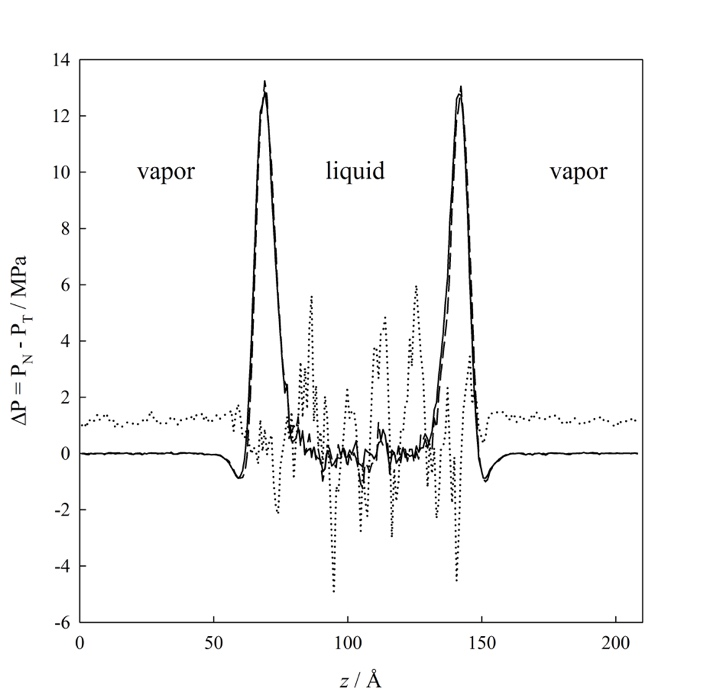
\includegraphics[width=0.5\textwidth]{gfx/image61.jpeg}
\caption{Time evolution of {${\Updelta}$}P = (P$_{\mathrm{N}}$-P$_{\mathrm{T}}$) vs $z$ profiles for the case of CO$_{2}$ (single Mie sphere) at 240 K at vapor \textendash{} liquid equilibria. ({\textbullet}{\textbullet}{\textbullet}) 18 ns, (${-}{-}$) 36 ns, and (\textemdash) 54 ns.}
\label{fig:17}
\end{figure}
From the pressure elements ${\langle}P_{N}$($z$)${\rangle}$
and ${\langle}P_{T}$($z$)${\rangle}$, the interfacial
tension, ${\gamma}$, between two bulk phases (\textit{e.g}., liquid
\textendash{} vapor or liquid \textendash{} liquid) can be calculated from Eq.
\ref{eq:hulshof}, which can be rewritten as:
\begin{equation}
\gamma=\int_{{\scriptstyle -\infty}}^{{\scriptstyle +\infty}}\left[\left\langle P_{zz}\left(z\right)\right\rangle -\frac{\left\langle P_{xx}\left(z\right)\right\rangle +\left\langle P_{yy}\left(z\right)\right\rangle }{2}\right]dz
  \label{eq:12}
\end{equation}

Fig. \ref{fig:18} displays the final average of ${\gamma}$
= ${\int}{\Updelta}{\langle}$P(z)${\rangle}$ dz along the interfacial
region, $z$, for vapor \textendash{} liquid \textendash{} vapor
interfaces. Two plateau regions are evident.
The first one corresponds to the first interfacial region (vapor \textendash{}
liquid) and the second correspond to the second interfacial region (liquid
\textendash{} vapor). The magnitude of the interfacial tension, ${\gamma}$, is
directly obtained from this figure, where the first plateau corresponds to
${\gamma}$ and the second plateau is the cumulative value of ${\gamma}$
(\textit{i.e.,} 2${\gamma}$ ). For the case illustrated in Fig. \ref{fig:18}, the IK
method (Eq. \ref{eq:12}) predicts ${\gamma}$ = 11.15 mN m$^{-1}$, which is similar to
the value obtained by Eq. \ref{eq:11}.
The recommended practice to evaluate the magnitude of ${\gamma}$ is to use the value
of the first plateau rather than the second value. The second value contains
all the accumulated error stemming from the liquid phase.
\begin{figure}
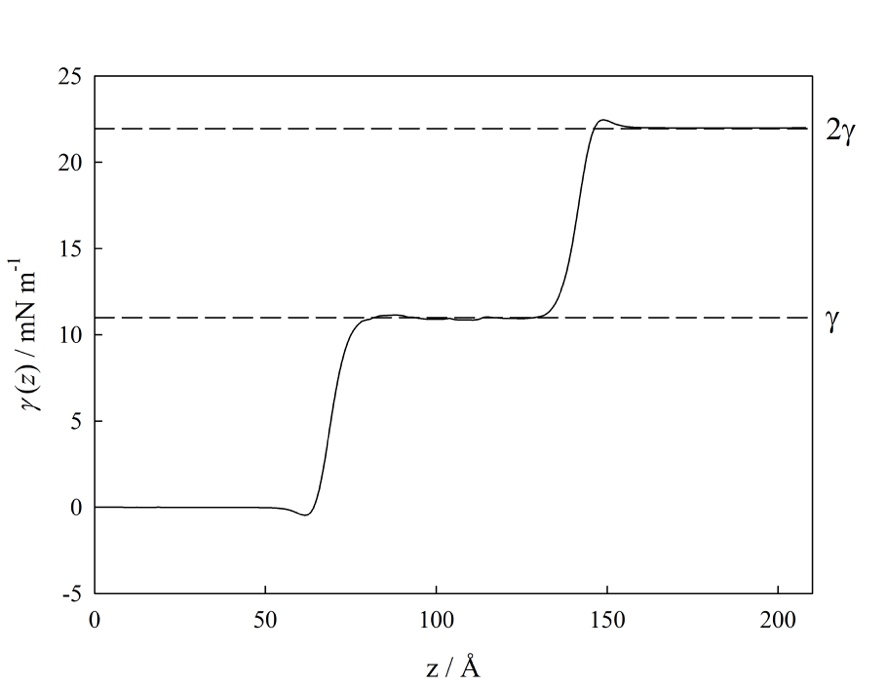
\includegraphics[width=0.5\textwidth]{gfx/image63.jpeg}
\caption{${\gamma}$ = ${\int}{\Updelta}{\langle}$P(z)${\rangle}$ dz along the interfacial region, $z$, for the case of CO$_{2}$ (single Mie sphere) at 240 K at vapor \textendash{} liquid equilibria.}
\label{fig:18}
\end{figure}

In summary, the evaluation of the magnitude of interfacial tension through the
mechanical route (or the pressure tensor) can be carried out by using two types
of averages over the diagonal element of the pressure tensor,
$P_{xx}$($z$), $P_{yy}$($z$), and
$P_{zz}$(z). The first approach evaluates these elements as an
ensemble average of the pressure tensor over the whole volume of the simulation
cell, ${\langle}P_{kk}{\rangle}$, whereas a second approach
calculates them by using an ensemble average of the upressure tensor along
discrete slabs in the $z$ coordinate,
${\langle}P_{kk}$($z$)${\rangle}$. The recommended practice to
compute the interfacial tension from the mechanical route is to use the latter 
method, which not only provides the interfacial tension value but also the
normal or equilibrium pressure. Citing \citet{holcomb1993} this route provides information of the time
evolution of these variables and can bring not only a picture of the
progression to equilibrium,  but also provides a way to establish a true
equilibrium condition and to evaluate some possible issues related with the
initial conditions used (\textit{e.g}., the positive slope of the first plateau
indicates that the initial density was lower than the expected value.) 

From a practical viewpoint, the IK tensor has been incorporated in all MD and
some MC codes (c.f. Table 1). However, most of them compute
${\langle}P_{kk}{\rangle}$, rather than
${\langle}P_{kk}$(z)${\rangle}$. To the best of our knowledge, only
the MD-LAMMPS and the MC-Gibbs codes include both
${\langle}P_{kk}{\rangle}$ and
${\langle}P_{kk}$(z)${\rangle}$ and also compute the interfacial
tension according to Eqs. \ref{eq:11} and \ref{eq:12}, respectively.

For the other MS codes, it is necessary to include a subroutine able to compute
$P_{kk}$ slabs by slabs along the $z$ coordinate. In the
supplementary information, DL\_POLY and HOOMD subroutines are included for the case of Mie
potential. 

\subsection{Thermodynamic route for the interfacial tension: Test area method}

The test area (TA) method provides a perturbative route to calculate the
interfacial tension, {${\gamma}$}. In order to evaluate Eq. \ref{eq:2}, an
equilibrated system (state 0) with interfacial area $A_{0}$
($A_{0}$ = 2 $L_{x,0}L_{y,0}$) is perturbed by an
infinitesimal change in the interfacial area. This perturbation translates the
system to a new state (perturbed state or state 1) that has the same volume as
the original state, but a different interfacial area. The new interfacial area
in state 1 is $A_{1}$, which is obtained using the following
transformations $L_{x,1} = L_{x,0} (1 + \upxi)^{1/2}$, and 
$L_{y,1} = L_{y,0} (1 + \upxi)^{1/2}$, where
{${\upxi}$} {\textless}{\textless} 1. Using this transformation,
$A_{1}$ = $A_{0}$ + {${\Delta}$}$A$ and
{${\Delta}$}$A$ = $L_{x,0}L_{y,0}$ {${\xi}$}. In
order to guarantee a constant volume condition, $L_{z}$ needs to
change from $L_{z,0}$ to $L_{z,1}$ = $L_{z,0}$ /(1
+ {${\upxi}$}). At each state (0 and 1), the configurational energy of the
system is calculated, and the difference {${\Delta}$}$U$
= $U_{1}{-}U_{0}$ is evaluated. The calculation of
{${\gamma}$} is carried out by both expanding (+ {${\Updelta}$}A) and
compressing (${-}${${\Updelta}$}A) the interfacial area, as illustrated
in Fig. \ref{fig:19}.

\begin{figure}
  \centering
	\begin{subfigure}{\linewidth} % width of left subfigure
    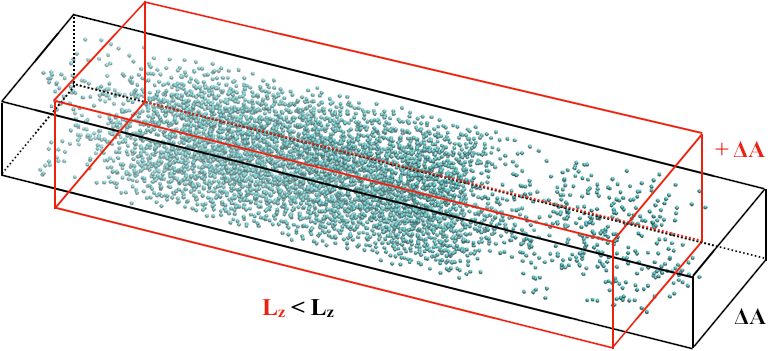
\includegraphics[width=0.9\textwidth]{gfx/image64.png}
	\end{subfigure}
	\begin{subfigure}{\linewidth} % width of left subfigure
    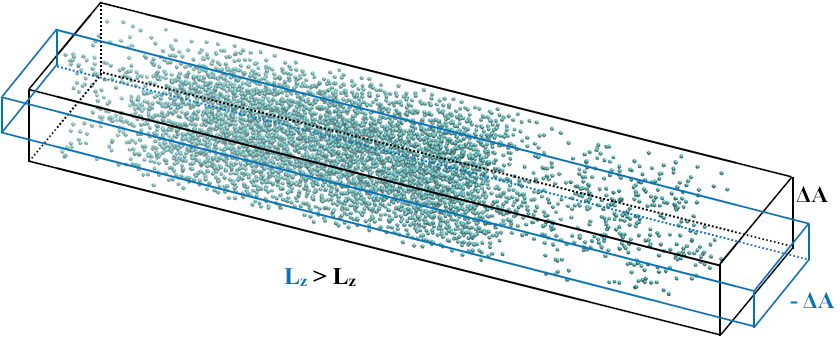
\includegraphics[width=0.9\textwidth]{gfx/image65.png}
	\end{subfigure}
\caption{Illustration of the area perturbation. Expanding (+ {${\Updelta}$}A) and compressing (${-}${${\Updelta}$}A) the interfacial area.}
\label{fig:19}
\end{figure}

The final value of {${\gamma}$} for a given {\textbar}{${\Updelta}$}A{\textbar}
is the result of the average over these two perturbations. A plot of the
corresponding Boltzmann average
${\langle}$exp(${-}${${\Updelta}$}U/k$_{\mathrm{B}}$T)${\rangle}_{0}$ as
a function of the perturbation {\textbar}{${\Updelta}$}A{\textbar} allows for
the calculation of the limiting value at {${\Updelta}$}A ${\rightarrow}$ 0. The
size of the perturbation {${\xi}$} is key in obtaining meaningful results. Too
small a perturbation will inevitably produce changes in energy which are of the
order of the machine precision, essentially noise, while too large of
a perturbation produces overlaps amongst the molecules and a deviation from the
expected linear regime. As a rule of thumb, it is advised to evaluate expansion
and compression paths for {${\xi}$} ranging from 10$^{{-}7}$ to 10$^{{-}2}$.
Fig. \ref{fig:20} illustrates the values of {${\gamma}$} obtained from MD using the TA
for the case of CO$_{2}$ + n-C$_{10}$H$_{22}$ mixture at 344.3 K and
$x_{1}$ = 0.448, where it is possible to observe that {${\gamma}$} is
constant in the range 10$^{-5}$ {\textless} {${\upxi}$} {\textless} 10$^{-3}$.
Using a value of {${\upxi}$} = 5 ${\times}$ 10$^{-4}$, the {${\gamma}$} = 8.46
mN m$^{-1}$.\citep{muller2009} 

\begin{figure}
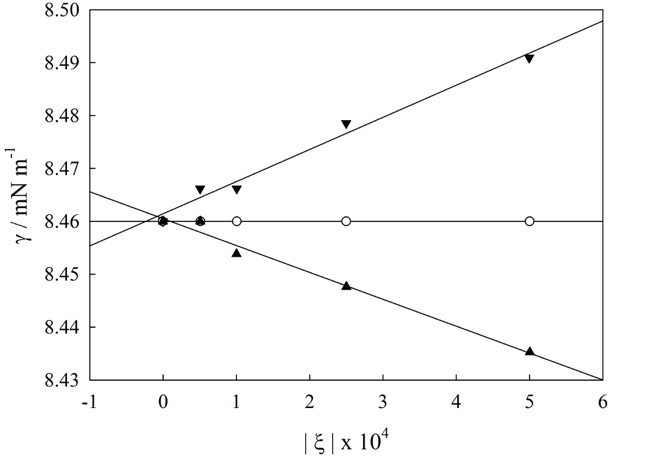
\includegraphics[width=0.45\textwidth]{gfx/image66.jpeg}
\caption{Values of {${\gamma}$} obtained from MD using the TA method at 344.3 K. The results are obtained for different values of the perturbation factor ${\upxi}$: $\blacktriangledown$, expansive perturbations, ${\upxi}$ {\textgreater} 0; $\blacktriangle$, compressive perturbations, ${\upxi}$ {\textless} 0; and O, average of the positive and negative perturbations.}
\label{fig:20}
\end{figure}

Further details concerning to the TA can be found in Ref.
\citep{gloor2005} for the methodological description, and some
application for TA can be found in Ref. \citep{muller2009}
for MD simulations and Refs. \citep{ghoufi2016,sampayo2010} for MC simulations.

The evaluation of interfacial tension through the thermodynamic route (or the
test area method) provides for a calculation of interfacial tension which is
distinct and independent of the mechanical route, and can be employed as a test
of consistency. Fig. \ref{fig:21} shows the interfacial tension of CO$_{2}$
+ n-C$_{10}$H$_{22}$ mixture at 344.3 K as a function of pressure. The MD
results have been obtained from IK, and TA methods and their results are
favourably compared to experimental data.
\begin{figure}
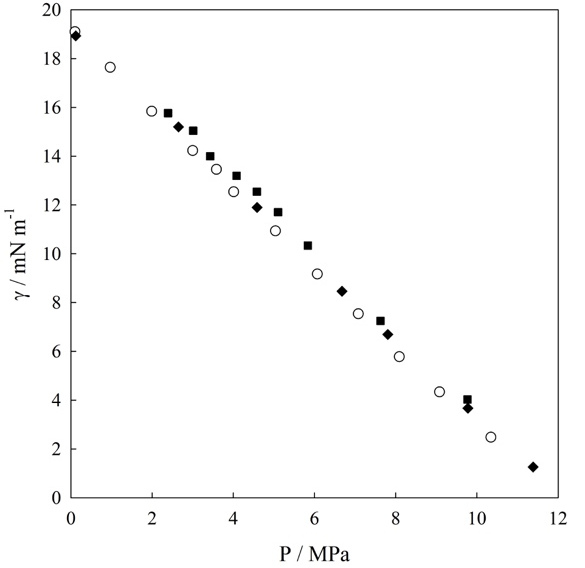
\includegraphics[width=0.8\linewidth]{gfx/image67.jpeg}
\caption{Interfacial tension for of CO$_{2}$ + n-C$_{10}$H$_{22}$ mixture at 344.3 K. O, Experimental \citep{mejia2014a}; ${\blacksquare}$, IK \citep{mejia2014a}; $\blacklozenge$, TA \citep{muller2009} .}
\label{fig:21}
\end{figure}
The TA method has been employed to study phenomena for which the mechanical route
is ill suited, such as in the determination of the interfacial tension of
discontinuous potentials \citep{gloor2005}
and drops and bubbles \citep{lau2015,sampayo2010}. The TA method will be a poor choice
for systems with long chain fluids. Here, the perturbative step is difficult to
carry out due to the periodic boundary conditions: operationally, the TA method
requires the removal of the periodic boundary conditions, the
expansion/compression of the simulation box and finally the recovery of the
boundary periodic conditions, steps which can be cumbersome for long chains.
Similarly, the method is only valid when one type of interface is present in the
simulation box, hence is unsuitable to study three-phase systems. 

\subsection{Other properties obtained from the interfacial tension}

By differentiation of the temperature dependence of the interfacial tension,
one can access both  the surface entropy (${\Updelta}s^{{\gamma}}$)
and surface enthalpy (${\Updelta}h^{{\gamma}}$) change of surface
formation, Eqs. \ref{eq:6} and \ref{eq:7}. This evaluation is carried out by a simple
numerical derivation of the MS results. As an example, Fig. \ref{fig:22} illustrates
${\Updelta}s^{\mathrm{{\gamma}}}$ and
${\Updelta}h^{\mathrm{{\gamma}}}$ change as a function of
temperature for selected n-alkanes.

Additionally, the interfacial tension as a function of temperature can be also
used to estimate the critical temperature for pure fluids. In this case, the
interfacial tension is correlated with the critical temperature by using the
scaling laws applied to the case of interfacial tension (see Eq. \ref{eq:8}).
This methodology is particular useful for the case of fluid with high of
critical temperatures where the experimental determination is unattainable 
(e.g. in the cases where the fluids suffer a thermal decomposition). Some examples
are the determination of the critical temperature of ionic liquids and
longer alkanes over C$_{16}$.

\begin{figure}[h]
	\centering
	\begin{subfigure}{0.68\linewidth} % width of left subfigure
    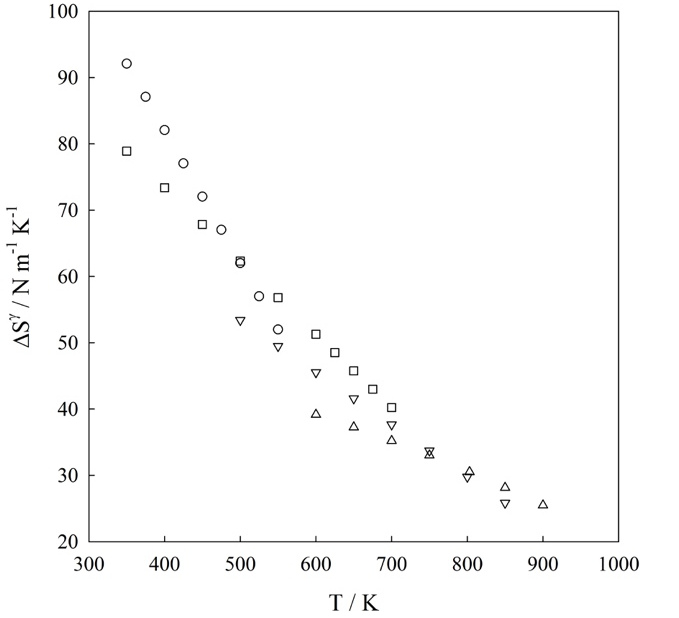
\includegraphics[width=1\textwidth]{gfx/image68.jpeg}
	\end{subfigure}
	\begin{subfigure}{0.68\linewidth} % width of left subfigure
    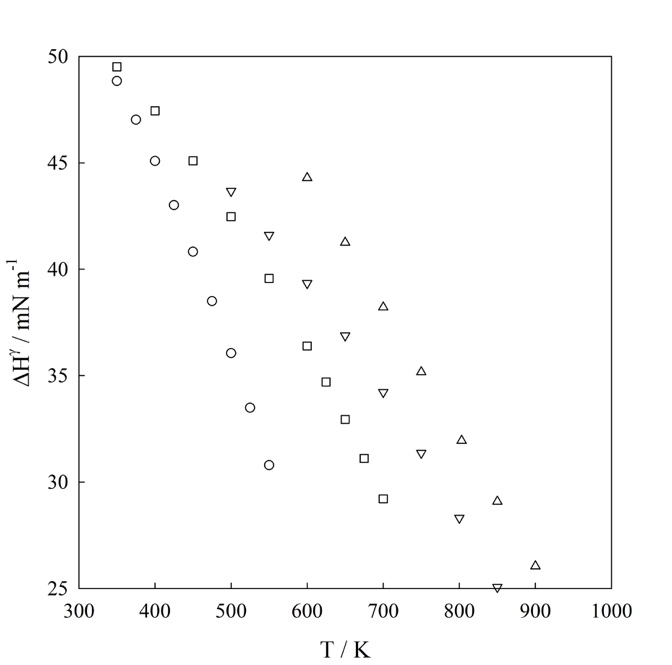
\includegraphics[width=1\textwidth]{gfx/image69.jpeg}
	\end{subfigure}
\caption{The surface entropy (${\Updelta}s^{\mathrm{{\gamma}}}$)
and surface enthalpy (${\Updelta}h^{\mathrm{{\gamma}}}$) change as
a function of temperature for selected n-alkanes. O, C$_{10}$H$_{22}$;
${\square}$, C$_{20}$H$_{42}$; ${\bigtriangleup}$, C$_{60}$H$_{122}$;
${\bigtriangledown}$, C$_{100}$H$_{202}$. (adapted from Ref. \citep{muller2011})}
\label{fig:22}
\end{figure}

\subsection{Statistics and errors}

An important aspect of reporting results is the evaluation of the errors
associated with the calculations. For the case of interfacial properties, it is
common to use block statistics where the information is averaged each
$n$ steps or cycles. In such a case, the production period is divided
into $n$ independent blocks. The statistical error is then deduced from
the standard deviation of the average ${\sigma}$/M$^{\mathrm{1/2}}$ where
${\sigma}$ is the variance of the block averages and $M$ is the number
of blocks, usually a number close to 10. For further details, the reader is
redirected to the \citet{allen2017}
and \citet{frenkel2002}
textbooks. Considering the advances in computer power (increased CPU and GPU speed,
massive parallelization of codes, etc.), an alternative route to evaluate the
statistics and deviation is to run the same MS a few times from different
initial states then use the final results for each simulation to calculate the
corresponding statistics, as if they were statistically different results.

Finally, it should be noted that several more advanced techniques are available
for estimating the statistical errors in interfacial properties. One approach
which is implemented in the GROMACS simulation software, and described in the
appendix of Ref. \citep{hess2002}, is to estimate the autocorrelation of the
pressure tensor components and to use this information in constructing an
optimal error estimate. Another technique which may be easier to implement is
the so-called ``jackknife'' technique, illustrated in Fig. \ref{fig:jackknife}.
In this approach, instead of dividing the production period into $n$ blocks,
one constructs a similar number of alternative blocks each of which comprise the entire data set
\textit{except for} the block in question.  This falls under the more general topic of
bootstrapping techniques, which are covered in statistics textbooks \citep{efron1982}.

\section{Common Pitfalls}

In this section, a summary of the most common pitfalls are presented as well as
their impact in the final results.

\begin{figure}
	\centering
  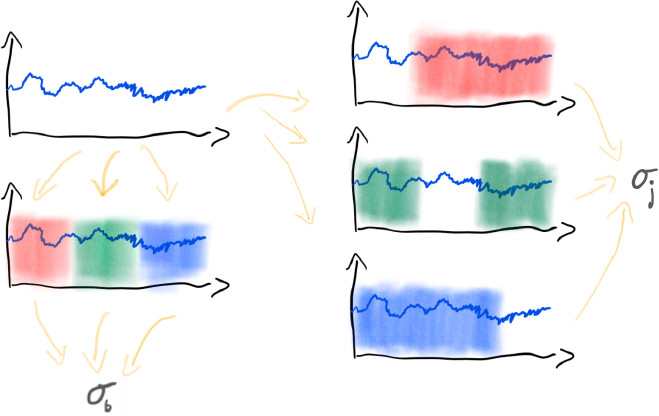
\includegraphics[width=\linewidth]{gfx/fig_jackknife.jpeg}
  \caption{Illustration of block averages giving an error estimate $\sigma_b$ (left) vs. the jackknife approach giving $\sigma_j$ (right).}
\label{fig:jackknife}
\end{figure}


\subsection{Inappropriate initial density}
\label{sec:init-dens}
A reasonable initial average of the expected liquid and vapor densities at the
simulation temperature is required for a two-phase simulation. The choice of
the initial density has an influence on the volume of each phase which will be
present at equilibrium.  If too few (too many) molecules are present in the
simulation box, \textit{i.e.} the global density is too low (high), the condensed
(vapor) phase will not be able to span the short dimensions of the box,
essentially condensing into a drop (bubble). This configuration (Fig.
\ref{fig:23}(a) ) does not allow the calculation of interfacial tensions, as
the heterogeneity of the system is incompatible with the assumptions made in
Eq. \ref{eq:hulshof}.

A reasonably sized liquid slab (Fig. \ref{fig:23}(c) ) should be wide enough to comfortably host a bulk liquid
region and its accompanying two interfaces. Too large of an initial density
creates problems of a different kind, such as the possible lack of a coexisting
vapor phase. The volume occupied by the vapor region must be larger than the
liquid region, as the statistics in the former phases are inherently poorer.
See Holcomb \textit{et al.} \citep{holcomb1993} for further discussions relating
to the use of inappropriate initial densities and the impact on the interfacial tension
calculations.

An associated error appears when the densities are chosen too close to the
actual phase boundaries, hence giving rise to the possibility of metastable
one-phase systems when otherwise a phase split is expected. $NVT$
simulations artificially enhance the stability of liquid phases.

\begin{figure}
	\centering
	\begin{subfigure}{0.3\textwidth} % width of left subfigure
    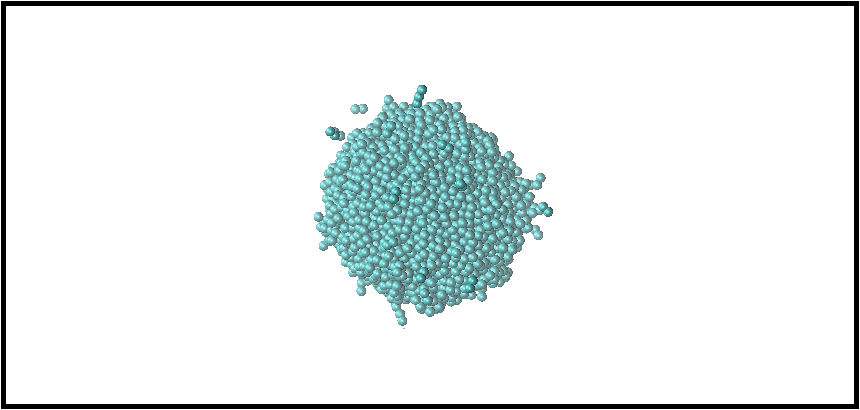
\includegraphics[width=1\textwidth]{gfx/Fig_23_a.png}
    \caption{Average density very low, no liquid slab}
	\end{subfigure}
	\begin{subfigure}{0.3\textwidth} % width of left subfigure
    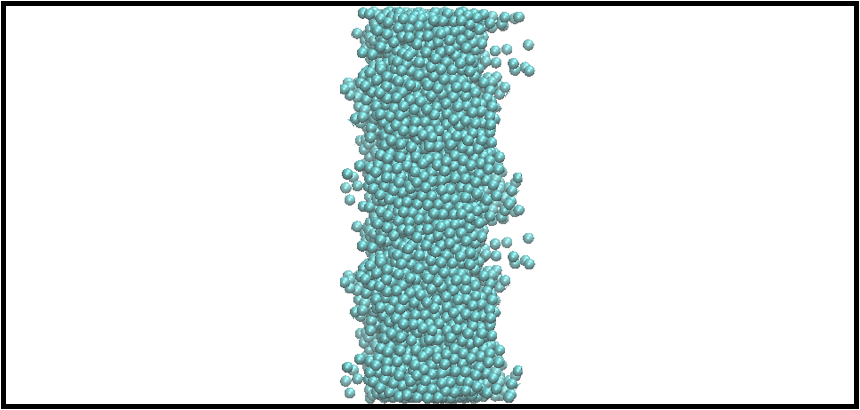
\includegraphics[width=1\textwidth]{gfx/Fig_23_b.png}
    \caption{Average density increased, but liquid slab too narrow}
	\end{subfigure}
	\begin{subfigure}{0.3\textwidth} % width of left subfigure
    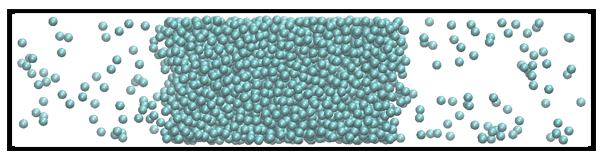
\includegraphics[width=1\textwidth]{gfx/Fig_23c.jpeg}
    \caption{Correct average density}
	\end{subfigure}
  \caption{Schematic illustration of common pitfalls in the initial density. (a) The overall density is too low
           and the condensed phase forms a droplet. (b) Increasing the density has removed the droplet.
           Now a slab spans the entire cell. However, the width of the liquid slab is too small and the
           interfacial regions play a significant role in the density profile. (c) A correct vapor-liquid ratio.}
\label{fig:23}
\end{figure}

\subsection{Selection of cutoff}

The value of the interfacial tension obtained from a force field is
particularly susceptible to the choice of cutoff, as exemplified in Fig. \ref{fig:11}.
The most visible effects of choosing a low values of the cutoff are the 
underprediction of the bulk liquid and vapor densities. Lower values of the liquid density
and higher values of vapor density directly impact the final value of the
interfacial tension ({${\gamma}$}  ${\simeq}$ (${\rho}^{\mathrm{L}}$
\textendash{} ${\rho}^{\mathrm{V}}$)$^{4}$).
%\begin{figure}
%	\centering
%	\begin{subfigure}{\linewidth} % width of left subfigure
%    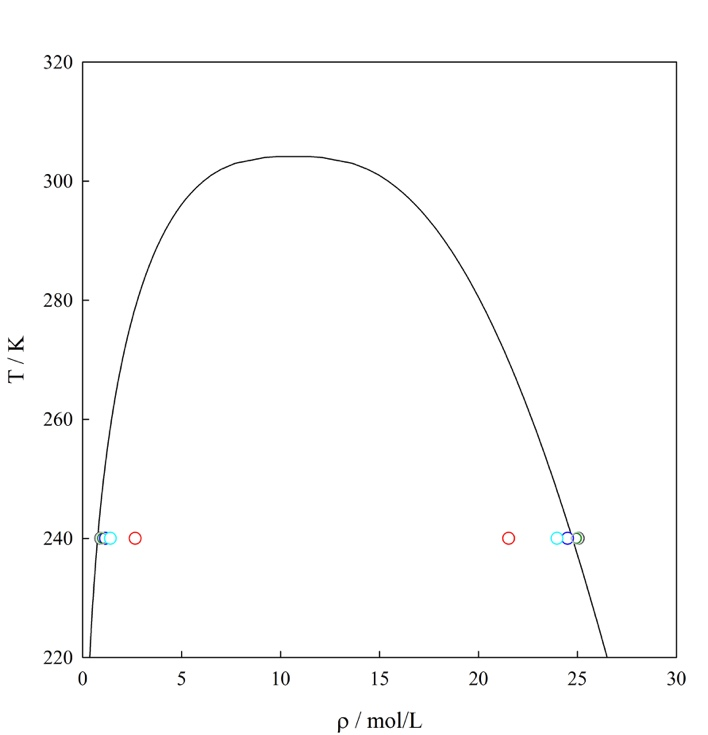
\includegraphics[width=1\textwidth]{gfx/image73.jpeg}
%    \caption{phase equilibria}
%	\end{subfigure}
%	\begin{subfigure}{\linewidth} % width of left subfigure
%    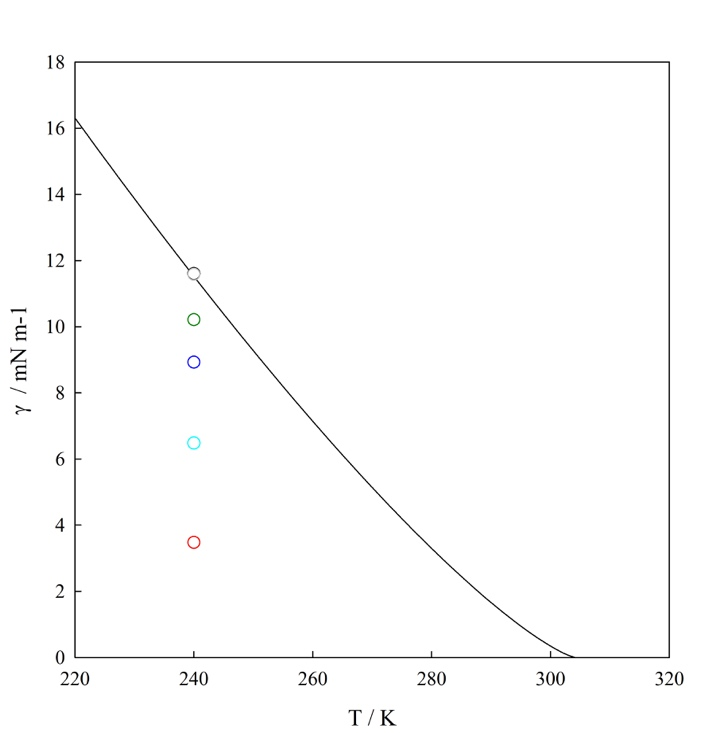
\includegraphics[width=1\textwidth]{gfx/image74.jpeg}
%    \caption{interfacial tension}
%	\end{subfigure}
%\caption{Illustration of the impact of cutoff in phase equilibrium ($T$
%\textendash{} {${\rho}$}) and interfacial tension ({${\gamma}$} \textendash{}
%$T$) for the case of CO$_{2}$ (single Mie sphere) at 240 K at vapor
%\textendash{} liquid equilibria. {\color{red}$\ocircle$}, $r_{c}$ = 2.0 {${\upsigma}$}; {\color{blue!40}$\ocircle$},
%$r_{c}$ = 2.5 {${\upsigma}$}; {\color{blue}$\ocircle$}, $r_{c}$ = 3.0
%{${\upsigma}$}; {\color{green}$\ocircle$}, $r_{c}$ = 4.0 {${\upsigma}$}; {\color{black!40}$\ocircle$}, $r_{c}$
%= 5.0 {${\upsigma}$}; $\ocircle$, $r_{c}$ = 6 {${\upsigma}$}. (\textemdash{})
%NIST \citep{lemmon2013}
%}
%\label{fig:24}
%\end{figure}
A key point however is to recognize that the parametrization of the force
fields is performed for a given cutoff-radius. Hence the choice of the cutoff
is generally not arbitrary, but dictated by the model employed. 
A related problem is associated with the choice of box dimensions; it is crucial to verify that the length of shortest side
( $L_{x}$ and $L_{y}$ ) be at least twice the cutoff radius.

\subsection{Poor temperature control/choice}

MS for interfacial properties of fluids are traditionally carried out in two
ensembles: $NVT$ and $NP_{zz}AT$, where the definition
of the temperature is required. However, the temperature range needs to be
selected very carefully to obtained trusty results of interfacial properties in
fluid-fluid interfaces. At low temperatures, the MS can display
cluster formation indicating the onset of a solid-like phase (see Fig. \ref{fig:25} (a) ).
At high temperatures (near to the critical state), the interfacial region will
be very diffuse causing a poor definition of both the bulk densities and the
interfacial region. In order to avoid these effects, it is recommnded to
carry out MS at temperatures from 0.5 {\textless} $T/T_{c}$
{\textless} 0.90.

\begin{figure}
	\begin{subfigure}{0.38\textwidth} % width of left subfigure
    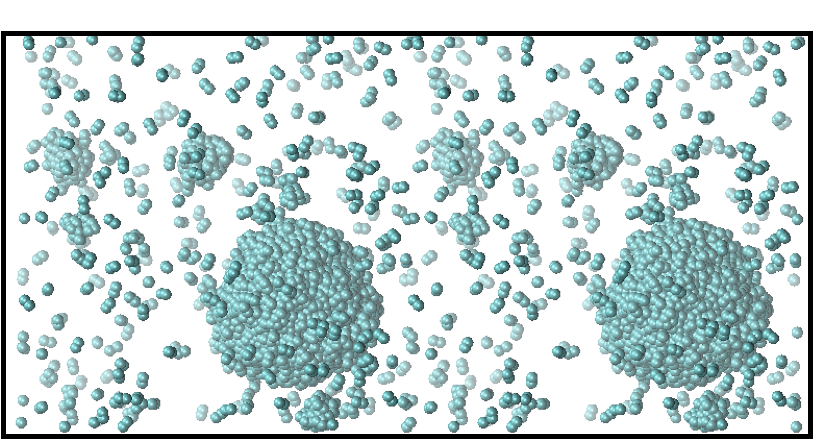
\includegraphics[width=1\textwidth]{gfx/image75.png}
    \caption{temperature close to the triple point}
	\end{subfigure}
	\begin{subfigure}{0.38\textwidth} % width of left subfigure
    \includegraphics[width=1\textwidth]{gfx/image76.png}
    \caption{temperature too close to critical state}
	\end{subfigure}
\caption{Illustration of poor temperature choices}
\label{fig:25}
\end{figure}

\subsection{Insufficiently long simulation} 

Based on the nature of the interfacial region, the MS needs to be run for
longer simulation time (\textit{i.e}., steps or cycles) than homogeneous fluids
to account for the longer diffusion times associated with phase rearrangement
and with the elongated shape of the simulation box. As a general guideline, the
simulation time for inhomogeneous fluids is three times the simulation time for
equivalent homogenous ones. Speedups can be achieved by using a thermal quench
first and then setting the thermostat to the selected simulation temperature
\citep{gelb2002}. Fig. \ref{fig:26} illustrates the case where insufficient equilibration time was
used.

\begin{figure}
\includegraphics[width=0.38\textwidth]{gfx/image77.png}
\caption{Illustration of insufficient equilibration time}
\label{fig:26}
\end{figure}

\subsection{Bugs and humans}\label{sec:bugs}

Our amazement at the speed in which modern computers can process data often
blinds us form the obvious statement that the computers are not (yet)
intelligent. Modern simulation codes will be composed of many thousands of
lines of code, usually contributed by authors spanning lengths of space and
time. Such collaboration is fruitful, but inevitably brings in the possibility
of making mistakes. The corresponding number of coding errors (bugs) in
a modern MS code is estimated to be in the upper 100's \citep{schappals2017},
even after extensive
testing. Many of these bugs will be inconsequential to a simulation, but some
might eventually creep into the results. More frequently however, human errors
and faulty implementations are the cause of fatal errors
\citep{wong2016}. In either case, it is important to validate in
detail an existing calculation (as provided in this manuscript) and to ensure
reproducibility and to minimize the pernicious effect of bugs and humans.  

\section{Conclusions}
Molecular simulation (MS) of interfacial properties of pure fluids and fluid
mixtures can be carried out by using Molecular Dynamics or Monte Carlo
schemes. However, the design of the molecular simulation and the route to
evaluate the interfacial properties plays a central role to obtain meaningful
results. This work provides a detailed guide to the design and analysis of
molecular simulations of inhomogeneous fluids to obtain the most important
interfacial properties of fluids.

For biphasic fluid systems (vapor-liquid and liquid-liquid), we suggest to
design the simulation box dimension using the average of the bulk phases at the
selected temperature (or at the lower value of temperature to be simulated)
with a total number of particles ranging from 5000 to 8000 sites, which can be
described as united atoms (UA) and coarse-grained atoms (CG). The ideal
simulation box is a parallelepiped cell with $L_{x}$
= $L_{y}$ {\textgreater} 10 ${\upsigma}_{\mathrm{max}}$ (the larger
molecular diameter) and $L_{z}$ = 3 to 10
$L_{x}$. The initial configuration of the molecules in
the simulation box should be assigned using their spatial positions in
a solidlike configuration without velocities nor forces. This initial
configuration should be first simulated at high temperature (above the critical
state) to homogenize the system. After a few steps, the final configuration is
quenched and used as the initial configuration to carry out the MS at the
desired temperature.

In order to reach an equilibrium state, we suggest using either the $NVT$ or
$NP_{zz}AT$ ensembles, where it is necessary to use
a thermostat to fix the temperature and/or a barostat to fix the pressure. A
very common choice is the Nos\'{e}-Hoover, which includes constants
({${\uptau}$}) to control the MS conditions. The range of these constant are
{${\uptau}$}$_{\mathrm{T}}$ are 0.5 to 2 ps, and
{${\uptau}$}$_{\mathrm{P}}$ are 0.2 to 1 ps, for temperature and pressure respectively. The simulation
length for inhomogeneous fluids needs to be larger than for homogeneous fluids.
For the case of MD, it is advised to use 10 to 15 ns for equilibration stage,
and 30 ns for the production state. For the case of mixtures, the system should
be equilibrated for 70 to 80 ns, and then another 150 ns for production. During
the production stage, it is advised to use block statistics to collect the
numerical results.

The actual calculation of interfacial tensions should be performed by dividing
the simulation box in $n$ slabs ($n{\simeq}$ 250 to 500) along
the $z-$direction. Within each slab, the density and the pressure tensor
(\textit{e.g}., using the Irving-Kirkwood formulation) and the results averaged
on a per-slab basis. These results will be used to calculate other interfacial
properties such as the relative Gibbs adsorption isotherm, surface entropy, and
surface enthalpy change and the interfacial tension.

Besides provided general recommendations for advantageous methods, this work also includes a worked-out
example and input files required to carry out the corresponding simulations to
reproduce selected results presented here.

\section*{Potentially Conflicting Interests}
The authors declare no conflicting interests.

\section*{Funding Information}
%%%%%%%
% Authors should acknowledge funding sources here. Reference specific grants.
%%%%%%%
A.M. acknowledges funding from Fondecyt (Chile) through Grant 1190107. E.A.M.
acknowledges funding from the Engineering and Physical Sciences Research
Council to the Molecular Systems Engineering group through Grant Nos.
EP/E016340, EP/I018212 and EP/J014958 and EP/R013152.
\AA{}.E. acknowledges funding from the Research Council of Norway (RCN) 
through the CLIMIT program (254813/E20), and through the HYVA project which 
is part of the Strategic Institute Programme of SINTEF Energy Research funded 
through the Basic Research Funding scheme of the Research Council of Norway.

\section*{Author Information}
\makeorcid

\appendix
\section{Checklist}
\label{checklist}
The recommendations of this manuscript are summarized in the checklist provided on the next page.

\section*{Supplementary Information: Attached code examples}
Some example codes are attached to this manuscript at \githubrepository.
These can be used for computing the interfacial properties of three systems: coarse-grained CO$_2$, coarse-grained decane, and finally a mixture of these.
The example codes are provided for DL\_POLY, HOOMD, and LAMMPS.

% This provides a checklist which
% - spans a full page
% - consists of multiple sub-checklists
% - exists on a separate page
% This style of checklist will be especially helpful if you want to encourage readers to print and use your checklist in practice, as they
% can easily print it without also printing other material from your manuscript. However, other styles of checklist are also possible (below).
\begin{Checklists*}[p!]
\begin{checklist}{Setup}
\textbf{Steps for setup the initial conditions}
\begin{itemize}
\item Select the $NVT$ ensemble \\
%\item Define the initial reference (or lower) simulation temperature ($T_{ref}$) (0.5 {\textless} $T/T_{c}$ {\textless} 0.90) \\
\item Select an appropriate total number of particles, $N_{T}$ (N$_{\mathrm{T}}$ = N$^{\mathrm{L}}$ + N$^{\mathrm{V}}$ ; N$^{\mathrm{L}}{\approx}$ 2000 to 5000; N$^{\mathrm{V}}{\approx}$ 1000 to 2000). For mixtures, check to see if there are enough molecules of each type to satisfy the expected compositions in each phase. \checkref{See Example 1 and Example 2.} \\
\item Choose a global density of the pure fluid or fluid mixture at $T_{ref}$ (\textit{i.e}., {${\rho}$} = ({${\rho}$}$^{\mathrm{L}}$ + {${\rho}$}$^{\mathrm{V}}$)/2). \checkref{See discussion around Fig. \ref{fig:23}.} \\
\item Calculate the simulation cell parameters (V = N$_{\mathrm{T}}$/ {${\rho}$} $= L_{x}L_{y}L_{z}$; $L_{x}$ = $L_{y}$ {\textgreater} 10 ${\sigma}_{\mathrm{max}}$;  $L_{z}{\approx}$ 3 to 10 $L_{x}$). \checkref{See Example 2.} \\
\item Choose a force field: UA or CG. \checkref{See Sec. \ref{sec:forcefields}.} \\
\item Select a cutoff compatible with the force field , otherwise choose $r_{c}{\geq}$ 6 ${\sigma}_{\mathrm{max}}$ . Verify that r$_{\mathrm{c}}^{\mathrm{max}}$ = $L_{x}$ /2). \checkref{See Sec. \ref{sec:cutoff}.} \\
\item Select a thermostat (e.g. Nos\'e-Hoover or better) with an appropriate constant (${\uptau}_{\mathrm{T}}{\approx}$ 0.5 to 1 ps). \checkref{See Sec. \ref{sec:thermostat}.} If using Verlet radii, choose delr = 1.5 ${\sigma}_{\mathrm{max}}$ \\
\item Set total Simulation Steps (SS ${\approx}$ 50000 to 100000). \\
\item Set a time step (${\Updelta}$t ${\approx}$ 0.01 to 0.003 ps) \\
\item Run MS at high temperature ($T_{H}$ {\textgreater}{\textgreater} $T_{C}$) to generate an initial configuration for the quench. \checkref{See Sec. \ref{sec:setup}.} \\
\end{itemize}
\end{checklist}

\begin{checklist}{Production run}
\textbf{Steps for running simulation at production conditions, after setup}
\begin{itemize}
  \item Set simulation ensemble: $NVT$ or $NP_{zz}AT$. \checkref{See Sec. \ref{sec:ensemble}.} \\
\item Set simulation temperature $T_{s}$ (0.5 {\textless} $T/T_{c}$ {\textless} 0.90)  \\
\item Set simulation pressure $P_{zz}$ (only for $NP_{zz}AT$) \\
\item Select a thermostat as before, and (only for $NP_{zz}AT$) a barostat with an appropriate constant ${\uptau}_{\mathrm{P}}{\approx}$ 0.5 to 1 ps, i.e. a barostat that maintains the desired $P_zz$ by scaling only the z-dimension of the box. \checkref{See Sec. \ref{sec:thermostat}.}\\
\item Set total Simulation Steps (SS ${\approx}$ 20 x 10$^{6}$ for pure fluids; 40 x 10$^{6}$ for fluids mixtures) of which the first third should be discarded as equilibration steps. \checkref{See Sec. \ref{sec:length}.} \\
\item Decide strategy for statistics, visualization, printing of configurations to disk (frequency to save) and post-processing ( if not included in main program). \checkref{See Sec. \ref{sec:post-proc}.}\\
\end{itemize}
\end{checklist}

%\begin{checklist}{Third list}
%\textbf{This is some further description.}
%\begin{itemize}
%\item First thing
%\item Also remember
%\item And finally
%\end{itemize}
%\end{checklist}

\end{Checklists*}

\clearpage


\bibliography{references}

%%%%%%%%%%%%%%%%%%%%%%%%%%%%%%%%%%%%%%%%%%%%%%%%%%%%%%%%%%%%
%%% APPENDICES
%%%%%%%%%%%%%%%%%%%%%%%%%%%%%%%%%%%%%%%%%%%%%%%%%%%%%%%%%%%%

%\appendix


\end{document}
